\documentclass[spanish]{article}

\usepackage{arxiv}

\usepackage[utf8]{inputenc} % allow utf-8 input
\usepackage[T1]{fontenc}    % use 8-bit T1 fonts
\usepackage{lmodern}        % https://github.com/rstudio/rticles/issues/343
\usepackage{hyperref}       % hyperlinks
\usepackage{url}            % simple URL typesetting
\usepackage{booktabs}       % professional-quality tables
\usepackage{amsfonts}       % blackboard math symbols
\usepackage{nicefrac}       % compact symbols for 1/2, etc.
\usepackage{microtype}      % microtypography
\usepackage{graphicx}

\title{Generación de red hidrográfica densa de República Dominicana a
partir de modelo digital de elevaciones de resolución media}

\author{
    José-Ramón Martínez-Batlle\orcidlink{0000-0001-9924-0327}
   \\
    Facultad de Ciencias \\
    Universidad Autónoma de Santo Domingo (UASD) \\
  Santo Domingo, República Dominicana \\
  \texttt{\href{mailto:joseramon@geografiafisica.org}{\nolinkurl{joseramon@geografiafisica.org}}} \\
   \And
    Michela Izzo Gioiosa\orcidlink{0000-0003-4835-3967}
   \\
    Directora Ejecutiva \\
    Guakia Ambiente \\
  Santo Domingo, República Dominicana \\
  \texttt{\href{mailto:michela.izzo@guakiambiente.org}{\nolinkurl{michela.izzo@guakiambiente.org}}} \\
  }

% Pandoc syntax highlighting
\usepackage{color}
\usepackage{fancyvrb}
\newcommand{\VerbBar}{|}
\newcommand{\VERB}{\Verb[commandchars=\\\{\}]}
\DefineVerbatimEnvironment{Highlighting}{Verbatim}{commandchars=\\\{\}}
% Add ',fontsize=\small' for more characters per line
\usepackage{framed}
\definecolor{shadecolor}{RGB}{248,248,248}
\newenvironment{Shaded}{\begin{snugshade}}{\end{snugshade}}
\newcommand{\AlertTok}[1]{\textcolor[rgb]{0.94,0.16,0.16}{#1}}
\newcommand{\AnnotationTok}[1]{\textcolor[rgb]{0.56,0.35,0.01}{\textbf{\textit{#1}}}}
\newcommand{\AttributeTok}[1]{\textcolor[rgb]{0.77,0.63,0.00}{#1}}
\newcommand{\BaseNTok}[1]{\textcolor[rgb]{0.00,0.00,0.81}{#1}}
\newcommand{\BuiltInTok}[1]{#1}
\newcommand{\CharTok}[1]{\textcolor[rgb]{0.31,0.60,0.02}{#1}}
\newcommand{\CommentTok}[1]{\textcolor[rgb]{0.56,0.35,0.01}{\textit{#1}}}
\newcommand{\CommentVarTok}[1]{\textcolor[rgb]{0.56,0.35,0.01}{\textbf{\textit{#1}}}}
\newcommand{\ConstantTok}[1]{\textcolor[rgb]{0.00,0.00,0.00}{#1}}
\newcommand{\ControlFlowTok}[1]{\textcolor[rgb]{0.13,0.29,0.53}{\textbf{#1}}}
\newcommand{\DataTypeTok}[1]{\textcolor[rgb]{0.13,0.29,0.53}{#1}}
\newcommand{\DecValTok}[1]{\textcolor[rgb]{0.00,0.00,0.81}{#1}}
\newcommand{\DocumentationTok}[1]{\textcolor[rgb]{0.56,0.35,0.01}{\textbf{\textit{#1}}}}
\newcommand{\ErrorTok}[1]{\textcolor[rgb]{0.64,0.00,0.00}{\textbf{#1}}}
\newcommand{\ExtensionTok}[1]{#1}
\newcommand{\FloatTok}[1]{\textcolor[rgb]{0.00,0.00,0.81}{#1}}
\newcommand{\FunctionTok}[1]{\textcolor[rgb]{0.00,0.00,0.00}{#1}}
\newcommand{\ImportTok}[1]{#1}
\newcommand{\InformationTok}[1]{\textcolor[rgb]{0.56,0.35,0.01}{\textbf{\textit{#1}}}}
\newcommand{\KeywordTok}[1]{\textcolor[rgb]{0.13,0.29,0.53}{\textbf{#1}}}
\newcommand{\NormalTok}[1]{#1}
\newcommand{\OperatorTok}[1]{\textcolor[rgb]{0.81,0.36,0.00}{\textbf{#1}}}
\newcommand{\OtherTok}[1]{\textcolor[rgb]{0.56,0.35,0.01}{#1}}
\newcommand{\PreprocessorTok}[1]{\textcolor[rgb]{0.56,0.35,0.01}{\textit{#1}}}
\newcommand{\RegionMarkerTok}[1]{#1}
\newcommand{\SpecialCharTok}[1]{\textcolor[rgb]{0.00,0.00,0.00}{#1}}
\newcommand{\SpecialStringTok}[1]{\textcolor[rgb]{0.31,0.60,0.02}{#1}}
\newcommand{\StringTok}[1]{\textcolor[rgb]{0.31,0.60,0.02}{#1}}
\newcommand{\VariableTok}[1]{\textcolor[rgb]{0.00,0.00,0.00}{#1}}
\newcommand{\VerbatimStringTok}[1]{\textcolor[rgb]{0.31,0.60,0.02}{#1}}
\newcommand{\WarningTok}[1]{\textcolor[rgb]{0.56,0.35,0.01}{\textbf{\textit{#1}}}}

% tightlist command for lists without linebreak
\providecommand{\tightlist}{%
  \setlength{\itemsep}{0pt}\setlength{\parskip}{0pt}}


% Pandoc citation processing
\newlength{\cslhangindent}
\setlength{\cslhangindent}{1.5em}
\newlength{\csllabelwidth}
\setlength{\csllabelwidth}{3em}
\newlength{\cslentryspacingunit} % times entry-spacing
\setlength{\cslentryspacingunit}{\parskip}
% for Pandoc 2.8 to 2.10.1
\newenvironment{cslreferences}%
  {}%
  {\par}
% For Pandoc 2.11+
\newenvironment{CSLReferences}[2] % #1 hanging-ident, #2 entry spacing
 {% don't indent paragraphs
  \setlength{\parindent}{0pt}
  % turn on hanging indent if param 1 is 1
  \ifodd #1
  \let\oldpar\par
  \def\par{\hangindent=\cslhangindent\oldpar}
  \fi
  % set entry spacing
  \setlength{\parskip}{#2\cslentryspacingunit}
 }%
 {}
\usepackage{calc}
\newcommand{\CSLBlock}[1]{#1\hfill\break}
\newcommand{\CSLLeftMargin}[1]{\parbox[t]{\csllabelwidth}{#1}}
\newcommand{\CSLRightInline}[1]{\parbox[t]{\linewidth - \csllabelwidth}{#1}\break}
\newcommand{\CSLIndent}[1]{\hspace{\cslhangindent}#1}

\usepackage{orcidlink} \usepackage{float} \usepackage[all]{nowidow} \usepackage[spanish]{babel} \usepackage{xcolor} \usepackage{tabu} \renewcommand\tablename{Tabla} \renewcommand\figurename{Figura} \newcommand{\beginsupplement}{ \setcounter{table}{0} \renewcommand{\thetable}{S\arabic{table}} \renewcommand\tablename{Tabla} \setcounter{figure}{0} \renewcommand{\thefigure}{S\arabic{figure}} \renewcommand\figurename{Figura} } \usepackage[hidelinks]{hyperref} \usepackage{xurl}
\begin{document}
\maketitle


\begin{abstract}
El resumen se colocará aquí.
\end{abstract}

\keywords{
    modelo digital de elevaciones
   \and
    análisis hidrológico
   \and
    procesamiento de datos geoespaciales
   \and
    hidrología computacional
  }

\hypertarget{introducciuxf3n}{%
\section{Introducción}\label{introducciuxf3n}}

El agua es un recurso crítico, que impulsa la economía y sostiene la
vida. A nivel global, pero especialmente en países que comparten islas
pequeñas, como República Dominicana (RD), la administración eficaz de
este recurso es esencial (Izzo et~al., 2010; Le, 2019; Lenderking
et~al., 2020; Lohmann, 2016; Mackay y Spencer, 2017; Roson, 2013). Sin
embargo, la gestión eficiente de los recursos hídricos puede verse
limitada por la falta de información precisa y completa sobre la red
hidrográfica. En este contexto, las fuentes actuales de información
geográfica, a pesar de su valor, presentan limitaciones en cuanto a su
resolución, cobertura y consistencia.

La red hidrográfica de RD digitalizada a partir del mapa topográfico
nacional a escala 1:50,000 (``MTN-50k'') (Instituto Cartográfico Militar
(ICM), 1989) ofrece una cobertura extensa pero carece de los detalles
necesarios para apoyar el análisis hidrológico. Por otro lado, los
estudios técnicos y multitemáticos de ámbito subnacional desarrollados
por el Instituto Nacional de Recursos Hidráulicos (INDRHI) de RD y otras
entidades, aunque son valiosas fuentes de información, utilizan
metodologías diversas, lo que limita la consolidación de una red
hidrográfica coherente a nivel nacional (CIDIAT y INDRHI, 1992;
Halcrow-COR Ing. S.A., 2002; INDRHI, 1996, 2012; INDRHI y AQUATER, 2000;
INDRHI y EPTISA, 2000; OEA y INDRHI, 1994; Rodríguez y Febrillet, 2006;
Secretaría de Estado de Medio Ambiente y Recursos Naturales, 2004;
SERCITEC y INDRHI, 2002).

Adicionalmente, las redes hidrográficas derivadas de modelos digitales
de elevaciones de baja resolución, como el Shuttle Radar Topography
Mission (SRTM) de 3 arco-segundos, normalmente presentan artefactos de
difícil depuración, además de que la longitud de los canales es siempre
más corta que la verdadera, resultando en redes poco densas (Jarvis
et~al., 2008; NASA JPL, 2013; NASA LP DAAC, 2000; National Aeronautics
and Space Administration y United States Geological Survey, 2009). Por
otro lado, el DEM SRTM de 1 arco-segundo (\textasciitilde30 metros)
garantiza la precisión mientras aumenta el detalle de elevación y parece
ser una de las fuentes más consistentes actualmente (Aziz y Rashwan,
2022). No obstante, nosotros hemos generado productos hidrográficos con
SRTM-DEM de 30 metros, y notamos que el nivel de detalle de la red es
bastante mejorable, sobre todo en áreas de montaña.

Desde 2014, Alaska Satellite Facility (ASF) inició la creación de
productos ALOS-PALSAR corregidos radiométricamente en función del
terreno (RTC), con el objetivo de mejorar la geometría y la
radiometría---coeficiente de retrodispersión por unidad de superficie
del frente de onda incidente, también conocido como \emph{gamma-nought},
\(\gamma^0\)---de las imágenes generadas por el sensor PALSAR (radar de
apertura sintética, banda L, con distintas polarizaciones y modos de
barrido) montado a bordo del satélite ALOS de la Agencia Espacial
Japonesa (JAXA) (ASF DAAC, 2014; JAXA/METI y ASF DAAC, 2015). ALOS fue
lanzado en 2006, pero luego de cinco años de servicio, perdió energía y
cesó la comunicación con el centro de control, aunque aún permanece en
órbita.

Para obtener los productos RTC, denominados propiamente como
``\emph{Hi-Res Terrain Corrected}'' o ``ALOS PALSAR RTC'', ASF requirió
de datos globales de elevación de la máxima resolución posible, para lo
cual empleó de forma preferente (según territorios) el SRTM de 1
arco-segundo. En el proceso fue necesario ajustar el espaciado de
píxeles del DEM fuente (\textasciitilde30 metros) para hacerlo coincidir
con el espaciado de píxel de las imágenes ALOS PALSAR (\textasciitilde{}
12.5 metros) usando una función de remuestreo (\emph{up-sampling}),
obteniéndose así un DEM de 12.5 metros (ASF DAAC, 2014; JAXA/METI y ASF
DAAC, 2015).

A pesar de que ASF advirtió que este DEM se empleó únicamente para
realizar la corrección radiométrica del terreno del producto derivado de
ALOS-PALSAR, y que no debería ser utilizado como fuente de elevación
precisa (ASF DAAC, 2014), lo cierto es que en países donde no se dispone
de DEM de mediana o alta resolución, se vuelve crucial indagar en el
potencial de cada nuevo producto disponible. Por esta razón, tras varias
pruebas iniciales en las que extrajimos redes de drenaje y elementos del
relieve a partir de este DEM, comprobamos que la red hidrográfica
obtenida tenía mucho mayor detalle que las redes generadas con cualquier
otra fuente disponible. Dado que la elevación precisa no es crucial en
nuestras aplicaciones, vimos un alto potencial en este DEM para realizar
aplicaciones de hidrología computacional, en concreto para la extracción
de redes densas con énfasis en áreas de montaña.

El propósito de este artículo es ofrecer nuevos datos para superar las
limitaciones de las redes hidrográficas existentes, desarrollando una
red densa de ríos, arroyos y cañadas---canales, talwegs---, con énfasis
en áreas montañosas donde la precisión es crítica, utilizando como
fuente el DEM servido con los productos ALOS PALSAR RTC de 12.5 metros
de resolución espacial. Nuestro segundo objetivo es optimizar el DEM,
reduciendo el ruido y asegurando su precisión hidrológica, a la vez que
mantenemos los elementos morfológicos significativos del terreno. El
tercer objetivo, no menos importante, es sistematizar el protocolo de
procesamiento con una metodología explícita, generando una base de
código abierto basada en software libre para el procesamiento de datos
de elevación e hidrología computacional, que ofrezca a personas
interesadas, especialmente a estudiantes, una referencia didáctica que
pueda aplicarse a fuentes de elevación similares.

Nuestro trabajo tiene potencial para suplir las demandas de información
sobre hidrografía de resolución fina, que es un aspecto crucial en
muchos estudios de modelación, análisis de riesgos, morfometría de
cuencas, entre otros. De manera particular, la hidrografía densa
generada por nosotros es idónea para mejorar la red estaciones
hidrométricas del país, la cual es limitada y afronta diversos desafíos
como muchas redes de este tipo a nivel global. Asimismo, nuestro trabajo
también podría contribuir información para acciones de conservación,
planificación y gestión de los recursos hídricos a nivel nacional (Burn,
1997; INDRHI, 2019; Mishra y Coulibaly, 2009; Mishra y Coulibaly, 2010).
Además, los datos generados pueden ser de gran valor para un amplio
rango de aplicaciones, incluyendo la planificación del uso del suelo, el
diseño de infraestructuras, la gestión de cuencas hidrográficas y la
modelización de escorrentía y erosión. A medida que nos enfrentamos a
los impactos del cambio climático y a la creciente escasez de agua,
esperamos que este trabajo sirva como una contribución significativa
para la gestión de los recursos hídricos en la República Dominicana
(Izzo et~al., 2010; Le, 2019; Lenderking et~al., 2020; Lohmann, 2016;
Mackay y Spencer, 2017; Roson, 2013).

\hypertarget{notas-sobre-terminologuxeda}{%
\subsection*{Notas sobre
terminología}\label{notas-sobre-terminologuxeda}}
\addcontentsline{toc}{subsection}{Notas sobre terminología}

La terminología utilizada para describir los distintos componentes de
los sistemas fluviales es un tema de continuo debate en el campo de la
geomorfología fluvial. Este debate suele estar intrínsecamente ligado a
la escala de análisis empleada; al variar la escala, incrementándola o
reduciéndola, los criterios empleados para delimitar las definiciones de
los elementos morfológicos, tienden a desdibujarse y/o a resultar
inconsistentes (García y Ojeda, 2011). Seleccionar el término apropiado
para describir la unidad topográficamente deprimida por donde fluye o
por donde podría circular el agua de escorrentía, es un desafío nada
despreciable. Este reto se intensifica cuando el idioma introduce
distintas connotaciones para términos similares, cuya traducción literal
puede generar confusión (como ocurre con \emph{channel} y canal en
inglés y español, respectivamente). (Anderson y Anderson, 2010;
Charlton, 2010; Gutiérrez Elorza, 2009; Pedraza Gilsanz, 1996).

Dado que las distintas acepciones y discrepancias en la terminología
superan el alcance del presente trabajo, fijaremos los términos que
utilizaremos de manera convencional. En este estudio, empleamos los
términos \emph{talweg} y canal de forma indistinta para referimos a la
unidad topográficamente deprimida por la que fluye, o podría fluir, la
corriente. En geomorfología, utilizamos la voz germánica \emph{talweg}
para referirnos a la línea imaginaria que traza la parte más baja de un
valle, razón por la cual también la hemos incluido entre los términos
usados (Foucault y Raoult, 1985). Es importante remarcar que nuestra
definición convencional no siempre se refiere a un curso fluvial
permanente, pues la circulación del agua está influenciada por múltiples
factores. Asimismo, cabe destacar que, a esta unidad geomorfológica en
sus distintas variantes hidrodinámicas y dimensionales, también se le
conoce con múltiples nombres en República Dominicana (en orden de mayor
a menor ``importancia''), como son río, arroyo o cañada, denominaciones
que también incorporamos en la redacción.

Finalmente, en nuestro en este trabajo también adoptamos los términos
curso, drenaje o corriente, especialmente cuando destacamos la presencia
de un flujo ya sea permanente, semipermanente o intermitente. Además,
para el análisis hortoniano de los sistemas fluviales, nos referimos al
sistema interconectado de canales, cursos, corrientes o drenajes con las
denominaciones ``red de drenajes'' o ``red hidrográfica''.

\hypertarget{materiales-y-muxe9todos}{%
\section{Materiales y métodos}\label{materiales-y-muxe9todos}}

\hypertarget{obtenciuxf3n-y-preprocesamiento-del-dem}{%
\subsection{Obtención y Preprocesamiento del
DEM}\label{obtenciuxf3n-y-preprocesamiento-del-dem}}

\begin{figure}[H]

{\centering 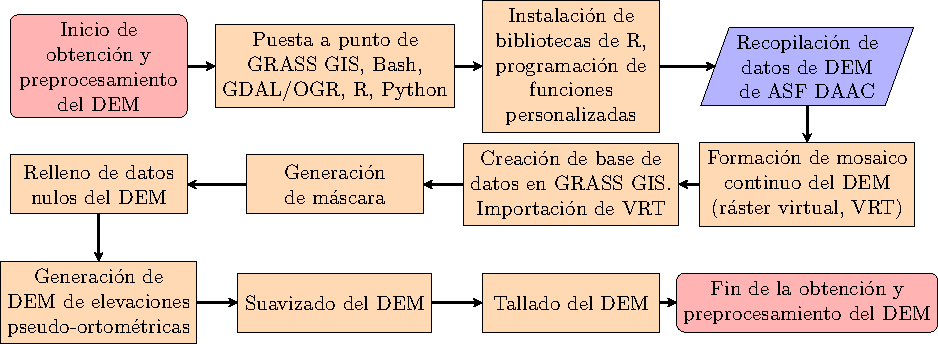
\includegraphics[width=0.8\linewidth]{resumen-obtencion-preprocesamiento-dem} 

}

\caption{Resumen gráfico de la obtención y preprocesamiento del DEM}\label{fig:obtencionpreprocdem}
\end{figure}

Iniciamos nuestro estudio valorando diversas herramientas para el
procesamiento de los datos. Debido a la gran variedad de complementos
que ofrece, junto con su alto rendimiento y la calidad de los resultados
que proporciona, decidimos utilizar GRASS GIS v8.2.0 para realizar la
mayor parte del procesamiento (Figura \ref{fig:obtencionpreprocdem}). La
implementación de su interfaz de línea de comandos (e.g.~interfaz basada
en texto), en nuestro caso Bash, garantizó la reproducibilidad de
nuestros procedimientos. Nos auxiliamos también de la biblioteca
GDAL/OGR, WhiteboxTools el entorno de programación estadística R y el
lenguaje de programación Python (GDAL/OGR contributors, 2022; GRASS
Development Team, 2023; Lindsay, 2018; R Core Team, 2023; Van Rossum y
Drake, 2009). Nuestro enfoque de reproducibilidad asegura que, sin
importar la fuente de datos empleada, el seguimiento del flujo de
trabajo es viable, manteniendo la integridad y coherencia del proceso de
análisis, sin menoscabo de la calidad del resultado final.

Asimismo, para facilitar nuestra labor, utilizamos una serie de
bibliotecas de R, además de funciones personalizadas escritas por
nosotros para agilizar y optimizar las tareas de limpieza y
representación de datos y mapas (Hijmans, 2023; O'Brien, 2023; Pebesma,
2018; Pebesma y Bivand, 2023; Wickham et~al., 2019; Xie, 2014, 2015,
2023; Zhu, 2021). El código reproducible usado en el estudio se puede
consultar en la sección \protect\hyperlink{infosupl}{Información
suplementaria}, así como los repositorios creados al efecto, donde
incluimos el código escrito y las direcciones para acceder a los datos
fuentes, entre otras utilidades.

Nos centramos en la fuente de datos, que en nuestro caso es el modelo
digital de elevaciones (DEM) servido con los productos \emph{Hi-Res
Terrain Corrected} de Alaska Satellite Facility (ASF) (ASF DAAC, 2014).
Este producto se descarga desde el Centro de Archivo Activo Distribuido
del Alaska Satellite Facility o ASF DAAC---una de las instalaciones
temáticas de la Administración Nacional de Aeronáutica y del Espacio de
los Estados Unidos, NASA---en forma de escenas o ``cuadros''
(\emph{tiles}), conteniendo dos imágenes de retrodispersión \(\gamma^0\)
(ca. 70x58 km cada una), una por cada polaridad, y el modelo digital de
elevaciones remuestreado con el que ASF realizó la corrección
radiométrica de terreno (ca. 80x70 km), objeto de nuestro estudio.

Cabe señalar que en un estudio de Aziz y Rashwan (2022), se evaluó la
precisión del DEM comparándolo con otras fuentes de elevación,
encontrándose un rendimiento relativamente bajo en varias pruebas. Sin
embargo, en el trabajo se utilizó el DEM sin preprocesar, lo cual
seguramente afectó el detectado bajo rendimiento. Consideramos que, a
pesar de los resultados de su comparativa, la alta resolución del DEM lo
convierte en una excelente opción para la extracción de redes de
drenaje, siempre que se apliquen filtros apropiados. Además, ASF señaló
en su documentación (ASF DAAC, 2014; JAXA/METI y ASF DAAC, 2015) que el
DEM usado en la RTC no es una fuente confiable de elevación, por lo que
el resultado obtenido por Aziz y Rashwan (2022) era más bien el
esperado.

Para conformar un mosaico continuo del DEM de República Dominicana,
seleccionamos y descargamos más de 40 escenas únicas de ALOS-PALSAR
desde el ASF DAAC (JAXA/METI y ASF DAAC, 2015), minimizando la
redundancia espacial y eligiendo las versiones más recientes,
conservando sólo 28 escenas distintas (Figura \ref{fig:mapaindice} y
Tabla \ref{tab:tablaindice}). Después, extrajimos los DEM
correspondientes de los archivos comprimidos y transformamos aquellos
proyectos en el huso 18N al 19N del sistema UTM. Posteriormente, creamos
un mosaico continuo (``sin costuras'') usando el formato de ráster
virtual.

\begin{figure}

{\centering 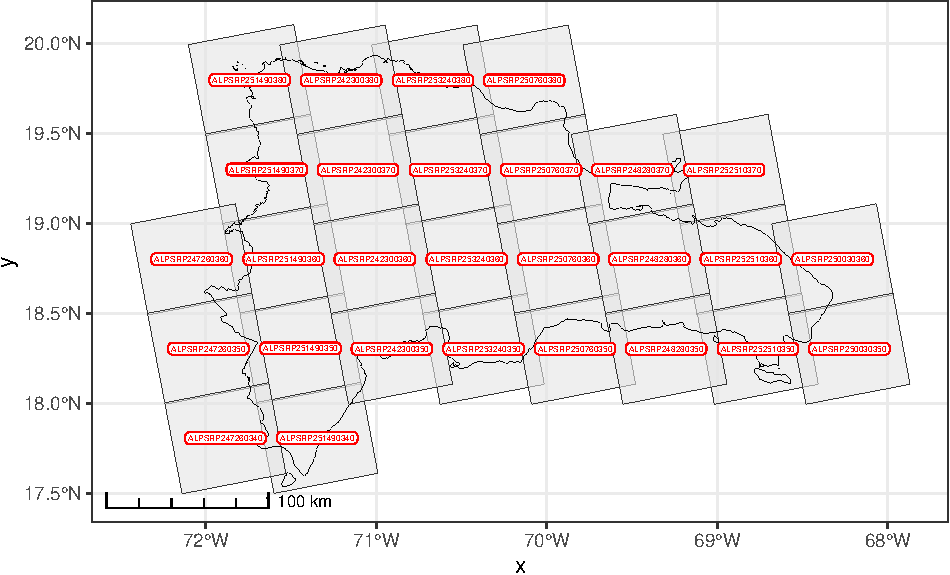
\includegraphics[width=0.8\linewidth]{preprint_files/figure-latex/mapaindice-1} 

}

\caption{Mapa índice de las 28 escenas usadas en la formación del DEM de República Dominicana, superponiendo las huellas (polígono de área con datos) de las escenas ALOS PALSAR RTC sobre el límite costero e internacional del país}\label{fig:mapaindice}
\end{figure}

Posteriormente, creamos una base de datos, con su correspondiente
localización, en GRASS GIS, nuestro software principal por su
eficiencia. Ocasionalmente recurrimos a otras herramientas como
WhiteboxTools y QGIS, siempre con el objetivo de optimizar el uso de los
recursos de hardware para obtener los resultados necesarios de manera
rápida (GRASS Development Team, 2023; Lindsay, 2018; QGIS Development
Team, 2021). Complementariamente, generamos una máscara de país en QGIS,
fusionando el límite oficial de la Oficina Nacional de Estadística con
fuentes en línea como GADM, OCHA y OpenStreetMap, y excluyendo
superficies de lagos naturales y embalses para facilitar el análisis de
cuencas endorreicas; este paso fue realizado de forma semimanual.
Posteriormente, importamos tanto el ráster virtual como la máscara a la
base de datos de GRASS GIS (Figura \ref{fig:demsinprocesar}).
Inmediatamente, aplicamos la máscara a la región activa para enfocar los
análisis sólo dentro del área de interés. (GADM, 2022; OCHA, 2022;
Oficina Nacional de Estadística (ONE), 2018; OpenStreetMap contributors,
2017; QGIS Development Team, 2021).

Dentro de la base de datos de GRASS, rellenamos los datos nulos del DEM
(Figura \ref{fig:demrelleno}), para luego suavizar el resultado
preservando morfologías con la herramienta
\emph{FeaturePreservingSmoothing} de WhiteboxTools (Figura
\ref{fig:demsuavizado}) (Lindsay, 2018; Lindsay et~al., 2019). Tras
esto, combinamos el DEM suavizado con el ráster de altura del geoide
EGM2008 mediante una simple suma algebraica para obtener alturas
pseudo-ortométricas, incrementando previamente la resolución del segundo
para acercarla ligeramente a la del primero.

A continuación, como último paso del preprocesamiento, tallamos el DEM
con una red preexistente de cursos largos de República Dominicana, un
paso clave en la generación de la hidrografía por métodos
computacionales, y que en inglés se conoce como \emph{stream burning}
(Lindsay, 2016). Primero creamos la red a partir de una selección de
ríos largos y permanentes, apoyados en imágenes satelitales (Google;
Airbus, CNES; Airbus, Landsat; Copernicus; Maxar Technologies; U.S.
Geological Survey, 2023), MTN-50K (Instituto Cartográfico Militar (ICM),
1989) y OpenStreetMap contributors (2017). Para representar ríos que que
llenan embalses, usamos sus trazados históricos para así mantener la
continuidad hidrológica (Figura \ref{fig:redcursoslargos}). Luego
realizamos el tallado del DEM probando tres algoritmos: \texttt{r.carve}
y \texttt{r.mapcalc} de GRASS GIS, y \texttt{FillBurn} de WhiteboxTools
(GRASS Development Team, 2022a; GRASS Development Team, 2022b, 2022c;
Larson et~al., 1991; Lindsay, 2018; Petrasova et~al., 2011; Saunders,
2000; Shapiro y Westervelt, 1994). Como criterio de selección
establecimos que el mejor algoritmo fuese aquel que lograra una mínima
alteración en el DEM, minimizando a la vez el tiempo de cómputo.
\texttt{r.carve} produjo un buen DEM tallado, aunque ocupó mucho tiempo
de cómputo, por lo que no la consideramos una herramienta adecuada para
iteraciones rápidas. Con \texttt{r.mapcalc} realizamos el tallado
mediante una simple álgebra de mapas (normalización, operaciones
booleanas, multiplicación), de donde obtuvimos un DEM poco alterado en
tiempo relativamente corto. Finalmente, probamos con la función
\texttt{FillBurn} de WhiteboxTools, la cual produjo un DEM tallado
sustancialmente alterado respecto del original, especialmente en las
áreas de karst con depresiones. Optamos por continuar nuestro flujo de
procesamiento con el DEM tallado por \texttt{r.mapcalc} (ver Figura
\ref{fig:demtallado}).

\hypertarget{procesamiento-de-hidrologuxeda-computacional}{%
\subsection{Procesamiento de hidrología
computacional}\label{procesamiento-de-hidrologuxeda-computacional}}

\hypertarget{resultados}{%
\section{Resultados}\label{resultados}}

\hypertarget{discusiuxf3n}{%
\section{Discusión}\label{discusiuxf3n}}

Por el énfasis que hemos puesto en la generación de la red hidrográfica
y la detallada metodología, nuestro trabajo es un artículo de datos y
metodológico a la vez.

Para lograr una rápida salida del trabajo, dejamos para futuras
investigaciones lo siguiente:

\begin{itemize}
\tightlist
\item
  Evaluación de precisión de la elevación.
\item
  Mejora de la hidrografía de las áreas llanas.
\item
  Análisis hortonianos exhaustivos.
\item
  Segregación de la red teórica y la red circulante.
\item
  Con respecto a la precisión posicional de la red, estimamos que es
  alta en sistemas montañosos no kársticos, y moderada en sistemas
  kársticos. En los sistemas kársticos en particular, nuestro mapa
  exhibe un grado ligeramente mayor de incertidumbre debido a la
  ausencia de un catálogo detallado y preciso de depresiones, como las
  dolinas, que en última instancia definen la topología y jerarquización
  de la red en estos relieves. Para subsanar esta carencia, generamos
  nuestro propio inventario de depresiones a partir del modelo de
  elevaciones seleccionado, aunque lo aplicamos con prudencia a la hora
  de determinar la ubicación de los sumideros reales donde el flujo se
  infiltra al karst. Es relevante mencionar que nuestra red podría
  presentar una precisión reducida en áreas urbanas y llanas, así como
  en terrenos con canales de riego. Sin embargo, este factor no impacta
  la relevancia de nuestro estudio, dado que se enfoca primordialmente
  en otros tipos de áreas.
\item
  En relación a las cuencas y redes de drenaje transfronterizas, es
  importante destacar que sólo se caracterizaron utilizando información
  la porción correspondiente al territorio dominicano. Como resultado,
  el orden de red máximo obtenido para estas redes podría no reflejar su
  orden real. Estas cuencas abarcan las de los ríos Artibonito,
  Pedernales y Masacre, además de varias cuencas menores dispersas a lo
  largo de la frontera. No obstante, una evaluación visual preliminar
  indica que la mencionada limitación no interfiere con el propósito de
  nuestro estudio. Además, en futuros trabajos, abordaremos estas
  cuencas de manera integral para proporcionar una visión más completa
  de su morfometría.
\item
  Para asegurar que los datos de elevación eran adecuados y precisos en
  términos de elevación, se debería validar el DEM con datos de puntos
  de verificación tomados con GNSS.
\end{itemize}

\hypertarget{financiamiento}{%
\section*{Financiamiento}\label{financiamiento}}
\addcontentsline{toc}{section}{Financiamiento}

Esta investigación recibió financiamiento del Banco Interamericano de
Desarrollo (BID), y fue apoyado por la ONG Guakía Ambiente y la
Universidad Autónoma de Santo Domingo (UASD).

\hypertarget{declaraciuxf3n-de-conflicto-de-intereses}{%
\section*{Declaración de conflicto de
intereses}\label{declaraciuxf3n-de-conflicto-de-intereses}}
\addcontentsline{toc}{section}{Declaración de conflicto de intereses}

El autor y la autora de este artículo declaran que no tienen ningún
conflicto de interés con el contenido de este artículo.

\hypertarget{disponibilidad-de-datos-scripts-y-cuxf3digo}{%
\section{Disponibilidad de datos, scripts y
código}\label{disponibilidad-de-datos-scripts-y-cuxf3digo}}

Los datos que respaldan los hallazgos de este estudio están disponibles
abiertamente en Zenodo en \url{https://doi.org/10.5281/zenodo.8146391}
(Martínez-Batlle y Izzo-Gioiosa, 2023). Los scripts utilizados para la
curación de datos, análisis y visualización están disponibles en esta
sección, así como en el repositorio de GitHub en
\url{https://github.com/geofis/red-hidrografica-densa-rd} y en Zenodo en
\url{} (\textbf{RELLENAR?}).

\newpage

\hypertarget{infosupl}{%
\section*{Información suplementaria}\label{infosupl}}
\addcontentsline{toc}{section}{Información suplementaria}

\beginsupplement

\hypertarget{suplemento-para-la-secciuxf3n-materiales-y-muxe9todos}{%
\subsection*{Suplemento para la sección Materiales y
Métodos}\label{suplemento-para-la-secciuxf3n-materiales-y-muxe9todos}}
\addcontentsline{toc}{subsection}{Suplemento para la sección Materiales
y Métodos}

\hypertarget{obtenciuxf3n-y-preprocesamiento-del-dem-1}{%
\subsubsection{Obtención y Preprocesamiento del
DEM}\label{obtenciuxf3n-y-preprocesamiento-del-dem-1}}

Los siguientes bloques de código cargan los paquetes de uso común a lo
largo de este cuaderno, así como funciones creadas por nosotros para
eficientizar las tareas de limpieza y representación de datos y mapas.
Igualmente, aprovechamos este bloque de código para declarar la ruta del
directorio donde se alojan los archivos fuente, la cual reaprovechamos
en distintas partes del código.

\begin{Shaded}
\begin{Highlighting}[]
\NormalTok{conflicted}\SpecialCharTok{::}\FunctionTok{conflict\_prefer}\NormalTok{(}\StringTok{"select"}\NormalTok{, }\StringTok{"dplyr"}\NormalTok{)}
\NormalTok{conflicted}\SpecialCharTok{::}\FunctionTok{conflict\_prefer}\NormalTok{(}\StringTok{"filter"}\NormalTok{, }\StringTok{"dplyr"}\NormalTok{)}
\FunctionTok{library}\NormalTok{(raster)}
\FunctionTok{library}\NormalTok{(sf)}
\FunctionTok{library}\NormalTok{(kableExtra)}
\FunctionTok{library}\NormalTok{(tidyverse)}
\FunctionTok{library}\NormalTok{(gdalUtilities)}
\FunctionTok{source}\NormalTok{(}\StringTok{\textquotesingle{}R/funciones.R\textquotesingle{}}\NormalTok{)}
\NormalTok{dem\_proc\_dir }\OtherTok{\textless{}{-}} \StringTok{\textquotesingle{}alos{-}palsar{-}dem{-}rd/dem/\textquotesingle{}}
\end{Highlighting}
\end{Shaded}

Descargamos 42 escenas ALOS PALSAR RTC, específicamente los \emph{Hi-Res
Terrain Corrected}, desde el Centro de Archivo Activo Distribuido (DAAC)
del \href{https://asf.alaska.edu/}{Alaska Satellite Facility (ASF)} (ASF
DAAC, 2014), para posteriormente depurarlas y seleccionar las más
idóneas para unirlas en un mosaico creado como ráster virtual. La
descarga la realizamos por lotes, usando un \emph{script} de Python
provisto por el propio ASF.

\begin{Shaded}
\begin{Highlighting}[]
\NormalTok{python download}\OperatorTok{{-}}\BuiltInTok{all}\OperatorTok{{-}}\DecValTok{2023}\OperatorTok{{-}}\DecValTok{0}\ErrorTok{4}\OperatorTok{{-}}\DecValTok{20\_00}\OperatorTok{{-}}\DecValTok{30}\OperatorTok{{-}}\FloatTok{00.}\ErrorTok{py}
\end{Highlighting}
\end{Shaded}

\begin{quote}
Al momento de realizarse esta investigación, la tendencia en el análisis
de datos geoespaciales apuntaba hacia enfoques basados en la nube, como
Google Earth Engine y Microsoft Planetary Computer. Nosotros usamos
regulamente estas plataformas en nuestras investigaciones, pero ciertos
algoritmos esenciales para el análisis hidrológico aún no se encuentran
disponibles en estos servicios. Por esta razón, nos vimos en la
necesidad de utilizar nuestros propios equipos informáticos (Intel(R)
Core(TM) i7-7700K CPU @ 4.20GHz, 64 GB de memoria RAM, unidad de estado
sólido NVMe, corriendo bajo Ubuntu 20.04) y, aunque conseguimos
paralelizar ciertos procesos, la mayoría de los algoritmos de
hidrolología computacional no utilizan eficientemente los múltiples
núcleos de los procesadores, resultando en una subutilización de la
capacidad de memoria y en procesamientos más lentos que los que
comúnmente se conseguirían en la nube.
\end{quote}

Identificamos las escenas necesarias para cubrir íntegramente la
República Dominicana, usando una búsqueda geográfica mediante polígono
delimitador en ASF. Dado que la misión del ALOS-PALSAR ofrece escenas de
distintas fechas para una misma área, las descargamos todas y
posteriormente excluimos del análisis las redundantes, conservando
siempre la más reciente. Utilizando el índice de huellas de escenas,
escribimos un pequeño programa para seleccionar las más recientes allí
donde hubiese redundancia. Con esto construimos un índice de DEM para
guiarnos durante la construcción del ráster virtual.

\begin{Shaded}
\begin{Highlighting}[]
\NormalTok{ind\_orig }\OtherTok{\textless{}{-}} \FunctionTok{invisible}\NormalTok{(}
  \FunctionTok{st\_read}\NormalTok{(}\StringTok{\textquotesingle{}alos{-}palsar{-}dem{-}rd/asf{-}datapool{-}results{-}2023{-}04{-}19\_08{-}31{-}26.geojson\textquotesingle{}}\NormalTok{,}
          \AttributeTok{quiet =}\NormalTok{ T)) }\SpecialCharTok{\%\textgreater{}\%} 
   \FunctionTok{rownames\_to\_column}\NormalTok{(}\StringTok{\textquotesingle{}fila\textquotesingle{}}\NormalTok{) }\SpecialCharTok{\%\textgreater{}\%} \FunctionTok{mutate}\NormalTok{(}\AttributeTok{fila =} \FunctionTok{as.integer}\NormalTok{(fila))}
\NormalTok{distancias }\OtherTok{\textless{}{-}}\NormalTok{ ind\_orig }\SpecialCharTok{\%\textgreater{}\%} \FunctionTok{st\_centroid}\NormalTok{() }\SpecialCharTok{\%\textgreater{}\%} \FunctionTok{st\_distance}\NormalTok{() }\SpecialCharTok{\%\textgreater{}\%}\NormalTok{ units}\SpecialCharTok{::}\FunctionTok{drop\_units}\NormalTok{()}
\NormalTok{distancias[}\FunctionTok{upper.tri}\NormalTok{(distancias, }\AttributeTok{diag =}\NormalTok{ T)] }\OtherTok{\textless{}{-}} \ConstantTok{NA}
\NormalTok{indices }\OtherTok{\textless{}{-}} \FunctionTok{which}\NormalTok{(distancias }\SpecialCharTok{\textless{}} \DecValTok{1000}\NormalTok{, }\AttributeTok{arr.ind =} \ConstantTok{TRUE}\NormalTok{)}
\NormalTok{duplicados }\OtherTok{\textless{}{-}} \FunctionTok{as.data.frame}\NormalTok{(indices) }\SpecialCharTok{\%\textgreater{}\%} 
  \FunctionTok{mutate}\NormalTok{(}\AttributeTok{dup\_id =} \DecValTok{1}\SpecialCharTok{:}\FunctionTok{nrow}\NormalTok{(indices)) }\SpecialCharTok{\%\textgreater{}\%} 
  \FunctionTok{pivot\_longer}\NormalTok{(}\SpecialCharTok{{-}}\NormalTok{dup\_id, }\AttributeTok{names\_to =} \StringTok{\textquotesingle{}tipo\textquotesingle{}}\NormalTok{, }\AttributeTok{values\_to =} \StringTok{\textquotesingle{}fila\textquotesingle{}}\NormalTok{) }\SpecialCharTok{\%\textgreater{}\%} 
  \FunctionTok{select}\NormalTok{(}\SpecialCharTok{{-}}\NormalTok{tipo)}
\NormalTok{seleccionados }\OtherTok{\textless{}{-}}\NormalTok{ duplicados }\SpecialCharTok{\%\textgreater{}\%}
  \FunctionTok{inner\_join}\NormalTok{(ind\_orig }\SpecialCharTok{\%\textgreater{}\%} \FunctionTok{select}\NormalTok{(fila, startTime) }\SpecialCharTok{\%\textgreater{}\%}\NormalTok{ st\_drop\_geometry) }\SpecialCharTok{\%\textgreater{}\%} 
  \FunctionTok{group\_by}\NormalTok{(dup\_id) }\SpecialCharTok{\%\textgreater{}\%} \FunctionTok{filter}\NormalTok{(startTime }\SpecialCharTok{==} \FunctionTok{max}\NormalTok{(startTime)) }\SpecialCharTok{\%\textgreater{}\%} \FunctionTok{pull}\NormalTok{(fila)}
\NormalTok{ind\_orig\_sel }\OtherTok{\textless{}{-}}\NormalTok{ ind\_orig }\SpecialCharTok{\%\textgreater{}\%}
  \FunctionTok{filter}\NormalTok{(}\SpecialCharTok{!}\NormalTok{fila }\SpecialCharTok{\%in\%}\NormalTok{ duplicados}\SpecialCharTok{$}\NormalTok{fila }\SpecialCharTok{|}\NormalTok{ fila }\SpecialCharTok{\%in\%}\NormalTok{ seleccionados) }\SpecialCharTok{\%\textgreater{}\%} 
  \FunctionTok{filter}\NormalTok{(centerLon }\SpecialCharTok{\textless{}} \SpecialCharTok{{-}}\FloatTok{72.1821}\NormalTok{)}
\end{Highlighting}
\end{Shaded}

\begin{Shaded}
\begin{Highlighting}[]
\NormalTok{ind\_orig\_sel }\SpecialCharTok{\%\textgreater{}\%} \FunctionTok{select}\NormalTok{(sceneName, startTime) }\SpecialCharTok{\%\textgreater{}\%} \FunctionTok{st\_drop\_geometry}\NormalTok{() }\SpecialCharTok{\%\textgreater{}\%}
  \FunctionTok{estilo\_kable}\NormalTok{(}\AttributeTok{titulo =} \FunctionTok{paste}\NormalTok{(}\StringTok{\textquotesingle{}Escenas ALOS{-}PALSAR usadas para generar un DEM de 12.5 m de}
\StringTok{                        resolución espacial de República Dominicana\textquotesingle{}}\NormalTok{))}
\end{Highlighting}
\end{Shaded}

\begin{table}[H]

\caption{\label{tab:tablaindice}Escenas ALOS-PALSAR usadas para generar un DEM de 12.5 m de
                        resolución espacial de República Dominicana}
\centering
\begin{tabu} to \linewidth {>{\raggedright}X>{\raggedright}X}
\toprule
sceneName & startTime\\
\midrule
ALPSRP253240380 & 2010-10-25 23:18:16\\
ALPSRP253240370 & 2010-10-25 23:18:08\\
ALPSRP253240360 & 2010-10-25 23:17:59\\
ALPSRP253240350 & 2010-10-25 23:17:51\\
ALPSRP252510370 & 2010-10-20 23:11:46\\
\addlinespace
ALPSRP252510360 & 2010-10-20 23:11:38\\
ALPSRP252510350 & 2010-10-20 23:11:30\\
ALPSRP251490380 & 2010-10-13 23:22:45\\
ALPSRP251490370 & 2010-10-13 23:22:36\\
ALPSRP251490360 & 2010-10-13 23:22:28\\
\addlinespace
ALPSRP251490350 & 2010-10-13 23:22:20\\
ALPSRP251490340 & 2010-10-13 23:22:12\\
ALPSRP250760380 & 2010-10-08 23:16:23\\
ALPSRP250760370 & 2010-10-08 23:16:15\\
ALPSRP250760360 & 2010-10-08 23:16:06\\
\addlinespace
ALPSRP250760350 & 2010-10-08 23:15:58\\
ALPSRP250030360 & 2010-10-03 23:09:44\\
ALPSRP250030350 & 2010-10-03 23:09:36\\
ALPSRP248280370 & 2010-09-21 23:14:21\\
ALPSRP248280360 & 2010-09-21 23:14:13\\
\addlinespace
ALPSRP248280350 & 2010-09-21 23:14:05\\
ALPSRP247260360 & 2010-09-14 23:25:03\\
ALPSRP247260350 & 2010-09-14 23:24:55\\
ALPSRP247260340 & 2010-09-14 23:24:47\\
ALPSRP242300380 & 2010-08-11 23:21:28\\
\addlinespace
ALPSRP242300370 & 2010-08-11 23:21:19\\
ALPSRP242300360 & 2010-08-11 23:21:11\\
ALPSRP242300350 & 2010-08-11 23:21:03\\
\bottomrule
\end{tabu}
\end{table}

En total, para cubrir el territorio de República Dominicana, necesitamos
28 de escenas únicas ALOS PALSAR RTC. Señalamos en este punto un detalle
relevante para el análisis hidrológico. Las escenas correspondientes a
la porción haitiana del río Artibonito, no las procesamos en este
estudio, a efectos de agilizar la producción de resultados. No obstante,
dicha tarea nos quedó pendiente para futuras investigaciones.

\begin{Shaded}
\begin{Highlighting}[]
\NormalTok{ind\_orig\_sel\_m }\OtherTok{\textless{}{-}}\NormalTok{ ind\_orig\_sel }\SpecialCharTok{\%\textgreater{}\%}
\NormalTok{  ggplot }\SpecialCharTok{+}
  \FunctionTok{geom\_sf}\NormalTok{(}\AttributeTok{alpha =} \FloatTok{0.6}\NormalTok{, }\AttributeTok{fill =} \StringTok{\textquotesingle{}grey90\textquotesingle{}}\NormalTok{, }\AttributeTok{color =} \StringTok{\textquotesingle{}grey20\textquotesingle{}}\NormalTok{, }\AttributeTok{size =} \FloatTok{0.5}\NormalTok{) }\SpecialCharTok{+}
  \FunctionTok{geom\_sf}\NormalTok{(}\AttributeTok{data =}\NormalTok{ pais, }\AttributeTok{fill =} \StringTok{\textquotesingle{}transparent\textquotesingle{}}\NormalTok{, }\AttributeTok{color =} \StringTok{\textquotesingle{}black\textquotesingle{}}\NormalTok{) }\SpecialCharTok{+}
  \FunctionTok{geom\_sf\_label}\NormalTok{(}\FunctionTok{aes}\NormalTok{(}\AttributeTok{label =}\NormalTok{ sceneName), }\AttributeTok{color =} \StringTok{\textquotesingle{}red\textquotesingle{}}\NormalTok{, }\AttributeTok{size =} \FloatTok{1.5}\NormalTok{,}
                \AttributeTok{label.padding =} \FunctionTok{unit}\NormalTok{(}\FloatTok{0.1}\NormalTok{, }\StringTok{"lines"}\NormalTok{), }\AttributeTok{alpha =} \FloatTok{0.9}\NormalTok{) }\SpecialCharTok{+}
  \FunctionTok{theme\_bw}\NormalTok{() }\SpecialCharTok{+} 
  \FunctionTok{theme}\NormalTok{(}\AttributeTok{plot.title =} \FunctionTok{element\_text}\NormalTok{(}\AttributeTok{size =} \DecValTok{11}\NormalTok{)) }\SpecialCharTok{+}
\NormalTok{  ggspatial}\SpecialCharTok{::}\FunctionTok{annotation\_scale}\NormalTok{(}\AttributeTok{style =} \StringTok{\textquotesingle{}ticks\textquotesingle{}}\NormalTok{)}
\end{Highlighting}
\end{Shaded}

Usando como referencia el índice de escenas seleccionadas, extrajimos
los DEM correspondientes, incluidos en formato GTiff dentro de los
archivos comprimidos (\texttt{.zip}). Este formato es proporcionado por
el Alaska Satellite Facility para minimizar el uso del ancho de banda
durante las descargas, lo que resulta beneficioso para el rendimiento de
sus servidores. A pesar de estar comprimidos, la descompresión de estos
archivos no supone un proceso largo o laborioso.

\begin{Shaded}
\begin{Highlighting}[]
\NormalTok{zip\_path }\OtherTok{\textless{}{-}} \StringTok{\textquotesingle{}alos{-}palsar{-}dem{-}rd/\textquotesingle{}}
\FunctionTok{sapply}\NormalTok{(ind\_orig\_sel}\SpecialCharTok{$}\NormalTok{fileName, }
       \ControlFlowTok{function}\NormalTok{(x)}
         \FunctionTok{unzip}\NormalTok{(}
           \AttributeTok{zipfile =} \FunctionTok{paste0}\NormalTok{(zip\_path, x),}
           \AttributeTok{exdir =} \FunctionTok{paste0}\NormalTok{(zip\_path, }\StringTok{\textquotesingle{}dem\textquotesingle{}}\NormalTok{), }\AttributeTok{junkpaths =}\NormalTok{ T,}
           \AttributeTok{files =} \FunctionTok{paste0}\NormalTok{(}\FunctionTok{gsub}\NormalTok{(}\StringTok{\textquotesingle{}.zip\textquotesingle{}}\NormalTok{, }\StringTok{\textquotesingle{}\textquotesingle{}}\NormalTok{, x), }\StringTok{\textquotesingle{}/\textquotesingle{}}\NormalTok{, }\FunctionTok{gsub}\NormalTok{(}\StringTok{\textquotesingle{}zip\textquotesingle{}}\NormalTok{, }\StringTok{\textquotesingle{}dem.tif\textquotesingle{}}\NormalTok{, x)))}
\NormalTok{       )}
\end{Highlighting}
\end{Shaded}

Todos los DEM fueron proporcionados por ASF en el sistema de coordenadas
Universal Transversal de Mercator (UTM). Sin embargo, los situados al
oeste fueron suministrados en el huso 18N. Identificamos estos DEM y los
transformamos al huso 19N, que es el que corresponde a nuestra área, con
el objetivo de generar un producto continuo. Para realizar esta
transformación, empleamos la herramienta \texttt{gdalwarp} de la
biblioteca GDAL (GDAL/OGR contributors, 2022).

\begin{Shaded}
\begin{Highlighting}[]
\NormalTok{dems\_orig\_path }\OtherTok{\textless{}{-}} \FunctionTok{list.files}\NormalTok{(}\AttributeTok{path =} \StringTok{\textquotesingle{}alos{-}palsar{-}dem{-}rd/dem\textquotesingle{}}\NormalTok{,}
                             \AttributeTok{pattern =} \StringTok{\textquotesingle{}*dem.tif\textquotesingle{}}\NormalTok{, }\AttributeTok{full.names =}\NormalTok{ T)}
\NormalTok{crs\_18n }\OtherTok{\textless{}{-}} \FunctionTok{names}\NormalTok{(}\FunctionTok{which}\NormalTok{(}\FunctionTok{sapply}\NormalTok{(dems\_orig\_path, }\ControlFlowTok{function}\NormalTok{(x)\{}
\NormalTok{  crs\_x }\OtherTok{\textless{}{-}} \FunctionTok{gdal\_crs}\NormalTok{(x)}
\NormalTok{  is\_z18 }\OtherTok{\textless{}{-}} \FunctionTok{grepl}\NormalTok{(}\StringTok{\textquotesingle{}zone 18N\textquotesingle{}}\NormalTok{, crs\_x[[}\StringTok{\textquotesingle{}wkt\textquotesingle{}}\NormalTok{]])}
\NormalTok{\})))}
\FunctionTok{sapply}\NormalTok{(crs\_18n, }\ControlFlowTok{function}\NormalTok{(x) }\FunctionTok{file.rename}\NormalTok{(}\AttributeTok{from =}\NormalTok{ x, }\AttributeTok{to =} \FunctionTok{gsub}\NormalTok{(}\StringTok{\textquotesingle{}.tif\textquotesingle{}}\NormalTok{, }\StringTok{\textquotesingle{}\_z18n.tif\textquotesingle{}}\NormalTok{, x)))}
\NormalTok{crs\_18n\_ren }\OtherTok{\textless{}{-}} \FunctionTok{list.files}\NormalTok{(}\AttributeTok{path =} \StringTok{\textquotesingle{}alos{-}palsar{-}dem{-}rd/dem\textquotesingle{}}\NormalTok{,}
                          \AttributeTok{pattern =} \StringTok{\textquotesingle{}z18n.tif\textquotesingle{}}\NormalTok{, }\AttributeTok{full.names =}\NormalTok{ T)}
\FunctionTok{sapply}\NormalTok{(crs\_18n\_ren, }\ControlFlowTok{function}\NormalTok{(x)\{}
  \FunctionTok{gdalwarp}\NormalTok{(}
  \AttributeTok{srcfile =}\NormalTok{ x,}
  \AttributeTok{dstfile =} \FunctionTok{gsub}\NormalTok{(}\StringTok{\textquotesingle{}\_z18n.tif\textquotesingle{}}\NormalTok{, }\StringTok{\textquotesingle{}.tif\textquotesingle{}}\NormalTok{, x), }
  \AttributeTok{t\_srs =} \StringTok{\textquotesingle{}EPSG:32619\textquotesingle{}}\NormalTok{, }\AttributeTok{overwrite =}\NormalTok{ T)\})}
\end{Highlighting}
\end{Shaded}

A efectos de eficientizar la manipulación del DEM, creamos un ráster
virtual (VRT) usando la herramienta \texttt{gdalbuildvrt} de la
biblioteca GDAL. Un ráster virtual es básicamente la abstracción de una
imagen que se genera \emph{on the fly}, creado a partir de un índice de
tamaño pequeño, en formato XML, que apunta a los archivos originales sin
moverlos ni alterarlos. Tienen las mismas prestaciones que las imágenes
guardadas permanentes guardadas en disco, por lo que con un ráster
virtual podemos visualizar un mosaico continuo o realizar análisis
intermedios, o evaluar un producto antes de crearlo de forma definitiva.
Se trata de un formato muy eficiente que ayuda a ahorrar espacio en
disco.

\begin{Shaded}
\begin{Highlighting}[]
\FunctionTok{gdalbuildvrt}\NormalTok{(}\AttributeTok{gdalfile =}\NormalTok{ dems\_orig\_path,}
             \AttributeTok{output.vrt =} \FunctionTok{paste0}\NormalTok{(}\FunctionTok{paste0}\NormalTok{(zip\_path, }\StringTok{\textquotesingle{}dem\textquotesingle{}}\NormalTok{), }\StringTok{\textquotesingle{}/dem\_seamless.vrt\textquotesingle{}}\NormalTok{),}
             \AttributeTok{resolution =} \StringTok{\textquotesingle{}highest\textquotesingle{}}\NormalTok{, }\AttributeTok{r =} \StringTok{\textquotesingle{}average\textquotesingle{}}\NormalTok{)}
\end{Highlighting}
\end{Shaded}

Posterioremente, creamos la base de datos y localización de GRASS GIS
usando como fuente de extensión y resolución el ráster virtual (GRASS
Development Team, 2023). Decidimos usar GRASS GIS a partir de este punto
para prácticamente todas las tareas de análisis geoespacial e
hidrológico, pues se trata de un software bastante eficiente en muchos
de sus complementos y algoritmos de serie (e.g.~rellenado de nulos). Sin
embargo, en pasos posteriores, alternamos el flujo de procesamiento con
otras herramientas, como WhiteboxTools (Lindsay, 2018). En todo caso,
nuestro criterio fue siempre aprovechar al máximo los recursos de
hardware y software disponibles para obtener los productos requeridos en
el menor tiempo posible.

\begin{Shaded}
\begin{Highlighting}[]
\CommentTok{\# Usando Bash, desde la ruta ./alos{-}palsar{-}dem{-}rd/dem}
\ExtensionTok{grass} \AttributeTok{{-}{-}text} \AttributeTok{{-}c}\NormalTok{ dem\_seamless.vrt ./grassdata}
\CommentTok{\# Para abrir luego de cerrada: grass grassdata/PERMANENT/}
\end{Highlighting}
\end{Shaded}

Luego creamos una máscara de país en QGIS (QGIS Development Team, 2021),
superponiendo el límite oficial obtenido desde la página de la
\href{https://www.one.gob.do/}{Oficina Nacional de Estadística (ONE)}, y
combinándolo con otras fuentes disponibles en línea, como
\href{https://gadm.org/}{GADM},
\href{https://data.humdata.org/dataset/cod-ab-dom}{Humanitarian Data
Exchange (OCHA)} y \href{https://www.openstreetmap.org}{OpenStreetMap}
(GADM, 2022; OCHA, 2022; Oficina Nacional de Estadística (ONE), 2018;
OpenStreetMap contributors, 2017). De la máscara, eliminamos las
superficies de máximas de lagos y lagunas no artificiales, pues nos
interesa procesar las cuencas endorreicas que drenan hacia ellos. No
obstante, los embalses no los incluimos en dicha superficie, dado que
necesitamos construir la jerarquía de red ignorando su presencia, es
decir, asumiendo como continuos todos los cursos fluviales. Sobre esta
máscara, creamos un área de influencia, para recortar el DEM con un
cierto ``acolchado'' que nos permitiera análizar sin dificultades las
áreas costeras y de frontera. La creación de esta máscara fue el único
paso que realizamos de forma semimanual, pues el resto del flujo de
procesamiento lo realizamos con algoritmo automáticos.

Posteriormente, importamos la máscara generada a la base de datos de
GRASS y la aplicamos. GRASS opera de forma eficiente, circunscribiendo
la aplicación de los algoritmos al área definida como máscara. Las áreas
fuera de ésta son excluidas, eficientizando los recursos y evitando
malgastar tiempo de CPU en áreas que ajenas al proyecto.

\begin{Shaded}
\begin{Highlighting}[]
\CommentTok{\# Importar máscara}
\ExtensionTok{v.import}\NormalTok{ input=mascara{-}1km.gpkg output=mascara\_1km}

\CommentTok{\# Fijar máscara}
\ExtensionTok{r.mask} \AttributeTok{{-}r}
\ExtensionTok{r.mask}\NormalTok{ vector=mascara\_1km}

\CommentTok{\# Ver ambiente}
\ExtensionTok{g.gisenv}
\CommentTok{\#\# GISDBASE=/media/jose/datos/alos{-}palsar{-}dem{-}rd/dem}
\CommentTok{\#\# LOCATION\_NAME=grassdata}
\CommentTok{\#\# MAPSET=PERMANENT}
\CommentTok{\#\# GUI=text}
\CommentTok{\#\# PID=1632142}
\end{Highlighting}
\end{Shaded}

Importamos el ráster virtual a la base de datos de GRASS GIS con la
herramienta \texttt{r.import}. Con este paso generamos un mapa ráster
dentro de la base de datos GRASS GIS, el cual es una realización con
celdas manipulables y a la que le podemos aplicar algoritmos ráster de
nuestra preferencia.

\begin{Shaded}
\begin{Highlighting}[]
\CommentTok{\# Importar DEM a región de GRASS}
\BuiltInTok{time}\NormalTok{ r.import }\AttributeTok{{-}{-}overwrite}\NormalTok{ input=dem\_seamless.vrt output=dem}
\CommentTok{\#\# real }

\CommentTok{\# Ver en lista (q para salir)}
\ExtensionTok{g.list}\NormalTok{ type=raster}
\end{Highlighting}
\end{Shaded}

\begin{figure}

{\centering \includegraphics[width=0.8\linewidth]{out/dem-sin-procesar} 

}

\caption{DEM sin procesar, representado como relieve sombreado. Nótesense los píxeles sin datos, destacados en color rojo (Los Patos-Ojeda-Paraíso, provincia Barahona, sudoeste de República Dominicana)}\label{fig:demsinprocesar}
\end{figure}

A continuación, rellenamos las celdas con valor nulo (sin datos) por
medio del eficiente complemento de GRASS \texttt{r.fill.nulls}. Lo
configuramos para rellenar píxeles nulos usando interpolación
\emph{spline} bilineal con regularización Tykhonov (\emph{spline} es un
método de descomposición de curvas en porciones descritas por
polinomios).

\begin{Shaded}
\begin{Highlighting}[]
\CommentTok{\# Rellenar vacíos}
\BuiltInTok{time}\NormalTok{ r.fillnulls }\AttributeTok{{-}{-}overwrite} \AttributeTok{{-}{-}verbose} \DataTypeTok{\textbackslash{}}
\NormalTok{  input=dem method=}\StringTok{"bilinear"} \DataTypeTok{\textbackslash{}}
\NormalTok{  tension=40 smooth=0.1 edge=3 npmin=600 segmax=300 lambda=0.01 }\DataTypeTok{\textbackslash{}}
\NormalTok{  output=dem\_relleno}
\CommentTok{\# Enviar mensaje al finalizar (ejecutar conjuntamente con anterior)}
\BuiltInTok{echo} \StringTok{"Job finished"} \KeywordTok{|} \ExtensionTok{mail} \AttributeTok{{-}s} \StringTok{"Job finished"}\NormalTok{ USUARIO@MAIL}
\CommentTok{\#\# real 10m11.925s}
\end{Highlighting}
\end{Shaded}

\begin{figure}

{\centering \includegraphics[width=0.8\linewidth]{out/dem-relleno} 

}

\caption{DEM sin procesar, representado como relieve sombreado. Los píxeles sin datos fueron eliminados (Los Patos-Ojeda-Paraíso, provincia Barahona, sudoeste de República Dominicana)}\label{fig:demrelleno}
\end{figure}

En el siguiente paso suavizamos el DEM preservando morfologías. Para
esto usamos la herramienta \emph{FeaturePreservingSmoothing} de
WhiteboxTools, la cual reduce la rugosidad generada por el ruido en el
DEM (Lindsay, 2018; Lindsay et~al., 2019). Para aplicar esta
herramienta, primero exportamos el DEM desde la base de datos de GRASS
GIS a archivo GeoTIFF, y posteriormente aplicamos el suavizado.
Finalmente, importamos el DEM suavizado nuevamente a la base de datos de
GRASS GIS para continuar el procesamiento en dicha aplicación.

\begin{Shaded}
\begin{Highlighting}[]
\CommentTok{\# Exportar a GTiff con compresión LZW}
\BuiltInTok{time}\NormalTok{ r.out.gdal }\AttributeTok{{-}{-}overwrite} \AttributeTok{{-}{-}verbose}\NormalTok{ createopt=}\StringTok{"COMPRESS=LZW,BIGTIFF=YES"} \DataTypeTok{\textbackslash{}}
\NormalTok{  input=dem\_relleno }\DataTypeTok{\textbackslash{}}
\NormalTok{  format=GTiff type=Float64 output=dem\_relleno.tif}
\CommentTok{\# Enviar mensaje al finalizar (ejecutar conjuntamente con anterior)}
\BuiltInTok{echo} \StringTok{"Job finished"} \KeywordTok{|} \ExtensionTok{mail} \AttributeTok{{-}s} \StringTok{"Job finished"}\NormalTok{ USUARIO@MAIL}
\CommentTok{\#\# real 0m58.924s}

\CommentTok{\# Comenzó a 23.20 de 22 de abril}
\BuiltInTok{time}\NormalTok{ \textasciitilde{}/WhiteboxTools\_linux\_amd64/WBT/whitebox\_tools }\DataTypeTok{\textbackslash{}}
  \AttributeTok{{-}{-}wd}\OperatorTok{=}\StringTok{\textquotesingle{}/media/jose/datos/alos{-}palsar{-}dem{-}rd/dem/\textquotesingle{}} \DataTypeTok{\textbackslash{}}
  \AttributeTok{{-}{-}filter}\OperatorTok{=}\NormalTok{25 }\AttributeTok{{-}{-}norm\_diff}\OperatorTok{=}\NormalTok{45 }\AttributeTok{{-}{-}num\_iter}\OperatorTok{=}\NormalTok{5 }\DataTypeTok{\textbackslash{}}
  \AttributeTok{{-}{-}run}\OperatorTok{=}\NormalTok{FeaturePreservingSmoothing }\AttributeTok{{-}{-}input}\OperatorTok{=}\StringTok{\textquotesingle{}dem\_relleno.tif\textquotesingle{}} \DataTypeTok{\textbackslash{}}
  \AttributeTok{{-}{-}output}\OperatorTok{=}\StringTok{\textquotesingle{}dem\_relleno\_suavizado.tif\textquotesingle{}} \AttributeTok{{-}v}
\CommentTok{\# Enviar mensaje al finalizar (ejecutar conjuntamente con anterior)}
\BuiltInTok{echo} \StringTok{"Job finished"} \KeywordTok{|} \ExtensionTok{mail} \AttributeTok{{-}s} \StringTok{"Job finished"}\NormalTok{ USUARIO@MAIL}
\CommentTok{\#\# real 9min46.103s}
\end{Highlighting}
\end{Shaded}

\begin{figure}

{\centering \includegraphics[width=0.8\linewidth]{out/dem-suavizado} 

}

\caption{DEM suavizado, representado como relieve sombreado. Nótese la conservación de las morfologías principales y la eliminación del ruido sobre éstas (Los Patos-Ojeda-Paraíso, provincia Barahona, sudoeste de República Dominicana)}\label{fig:demsuavizado}
\end{figure}

\begin{Shaded}
\begin{Highlighting}[]
\BuiltInTok{time}\NormalTok{ r.import input=dem\_relleno\_suavizado.tif output=dem\_suavizado}
\BuiltInTok{echo} \StringTok{"Job finished"} \KeywordTok{|} \ExtensionTok{mail} \AttributeTok{{-}s} \StringTok{"Job finished"}\NormalTok{ USUARIO@MAIL}
\CommentTok{\#\# real 0m21.593s}
\end{Highlighting}
\end{Shaded}

A continuación, usamos el ráster de altura de geoide de La Española a 1
minuto de resolución (EGM2008) para obtener alturas pseudo-ortométricas,
por medio de una suma algebraica simple de este ráster y el DEM
suavizado en GRASS GIS con la herramienta \texttt{r.mapcalc}. Sin
embargo, previamente fue necesario aumentar la resolución del ráster de
altura del geoide antes de realizar la suma. Para esto, usamos
\texttt{r.resamp.rst} (evaluamos una segunda alternativa con el
complemento \texttt{r.resamp.interp} y, aunque realizó el trabajo
eficientemente, eliminó muchas áreas limítrofes, por lo que preferimos
no utilizarlo).

\begin{Shaded}
\begin{Highlighting}[]
\CommentTok{\# Importar DEM a región de GRASS}
\ExtensionTok{r.import} \AttributeTok{{-}{-}overwrite}\NormalTok{ input=egm2008{-}1\_espanola.tif output=egm2008\_1min}

\CommentTok{\# Ver en lista (q para salir)}
\ExtensionTok{g.list}\NormalTok{ type=raster}

\CommentTok{\# Ver atributos de la región}
\ExtensionTok{g.region} \AttributeTok{{-}p}

\CommentTok{\# Alternativa 1. Usando r.resamp.rst. Más eficiente y precisa}
\CommentTok{\# Fijar la región al geoide importado}
\ExtensionTok{g.region}\NormalTok{ raster=egm2008\_1min }\AttributeTok{{-}ap}
\CommentTok{\# Realizar la interpolación}
\ExtensionTok{r.resamp.rst} \AttributeTok{{-}{-}overwrite}\NormalTok{ input=egm2008\_1min ew\_res=50 ns\_res=50 elevation=egm2008\_hires}
\BuiltInTok{echo} \StringTok{"Job finished"} \KeywordTok{|} \ExtensionTok{mail} \AttributeTok{{-}s} \StringTok{"Job finished"}\NormalTok{ USUARIO@MAIL}
\CommentTok{\#\# real }
\CommentTok{\# Fijar región a nuevo geoide}
\ExtensionTok{g.region}\NormalTok{ raster=egm2008\_hires }\AttributeTok{{-}ap}

\CommentTok{\# Alternativa 2. Usando r.resamp.interp. También eficiente, pero eliminar áreas de borde}
\CommentTok{\# g.region res=50 {-}ap}
\CommentTok{\# r.resamp.interp {-}{-}overwrite input=egm2008\_1min \textbackslash{}}
\CommentTok{\#  output=egm2008\_hires method=bilinear}

\CommentTok{\# Exportar para explorar visualmente}
\CommentTok{\# r.out.gdal {-}{-}overwrite {-}{-}verbose createopt="COMPRESS=LZW" \textbackslash{}}
\CommentTok{\#  input=egm2008\_hires \textbackslash{}}
\CommentTok{\#  format=GTiff type=Float64 output=egm2008\_hires.tif}

\CommentTok{\# Volver a resolución de DEM rellenado y suavizado}
\ExtensionTok{g.region}\NormalTok{ raster=dem\_suavizado }\AttributeTok{{-}ap}

\CommentTok{\# Aplicar álgebra de mapas}
\ExtensionTok{r.mapcalc} \AttributeTok{{-}{-}overwrite} \StringTok{"dem\_pseudo\_ortometrico = dem\_suavizado {-} egm2008\_hires"}

\CommentTok{\#Estadísticos univariados}
\ExtensionTok{r.univar}\NormalTok{ dem\_pseudo\_ortometrico}
\CommentTok{\# n: 306462417}
\CommentTok{\# minimum: {-}51.4456}
\CommentTok{\# maximum: 3102.34}
\CommentTok{\# range: 3153.79}
\CommentTok{\# mean: 403.703}
\CommentTok{\# mean of absolute values: 403.858}
\CommentTok{\# standard deviation: 487.27}
\CommentTok{\# variance: 237432}
\CommentTok{\# variation coefficient: 120.7 \%}
\CommentTok{\# sum: 123719658638.311}
\end{Highlighting}
\end{Shaded}

El resumen estadístico proporcionado por la herramienta
\texttt{r.univar} de GRASS GIS, usando la máscara ajustada a los límites
costeros e internacional del país, informa que la elevación mínima es
-51.5 m, mientras que la máxima es 3102.34 m, para un rango de casi 3154
m. El valor mínimo probablemente no está bien recogido, debido a que la
máscara empleada podría estar eliminando elevaciones muy bajas en el
área de la Hoya de Enriquillo. La elevación media, considerando tanto
los negativos como los positivos, es de aproximadamente 404 m, con
desviación estándar de 487 m y coeficiente de variación de 121\%.
Remarcamos que, aunque ASF advierte de no usar este modelo para fines de
elevación, el valor máximo se ajusta bastante a la elevación máxima
conocida en República Dominicana, que es el pico Duarte (Instituto
Geográfico Nacional, 2022).

\begin{figure}

{\centering \includegraphics[width=0.8\linewidth]{out/perfiles-dem/los-patos} 

}

\caption{Alturas respecto de geoide EGM08 ($\sim$ortométrica) y sobre elipsoide WGS84, de un transecto descendente desde Bahoruco Oriental al Mar Caribe (Los Patos-Ojeda-Paraíso, provincia Barahona, sudoeste de República Dominicana)}\label{fig:alturasgeoideelipsoide}
\end{figure}

A continuación, efectuamos el procedimiento de tallado o grabado de una
red preexistente sobre el DEM, conocido como \emph{stream burning}
(Lindsay, 2016). Con este procedimiento, logramos que los píxeles del
DEM intersectados con el vectorial de la red preexistente, adquieran un
valor muy bajo respecto de su entorno, para asegurar que los algoritmos
automáticos de análisis hidrológico dirijan el flujo a través de los
lechos de ríos establecidos. El tallado es particularmente útil, incluso
esencial, en áreas planas, ya que ayuda a los algoritmos autómáticos a
producir redes hidrográficas más realistas y topológicamente correctas.
Sin embargo, su aplicación de requiere de una cuidadosa selección de la
red preexistente a tallar. Para crearla, usamos una red de drenaje de
cursos fluviales seleccionados, que incluyó sólo los de gran longitud,
comúnmente ríos permamentes, de lecho ancho y claramente establecidos.
Nos apoyamos en imágenes satelitales (Google; Airbus, CNES; Airbus,
Landsat; Copernicus; Maxar Technologies; U.S. Geological Survey, 2023)
y, ocasionalmente, en el MTN-50K (Instituto Cartográfico Militar (ICM),
1989). Complementamos con OpenStreetMap contributors (2017), ya que este
servicio provee información vectorial de fácil acceso y precisa. El
resultado consistió en una red de cursos largos seleccionados de
República Dominicana, representada por los ríos Artibonito, Yaque del
Norte, Yuna, Yaque del Sur, varios ríos del extremo meridional de la
cordillera Central y del borde sudoriental del país, así como algunos
ríos seleccionados de la cordillera Septentrional.

\begin{figure}

{\centering 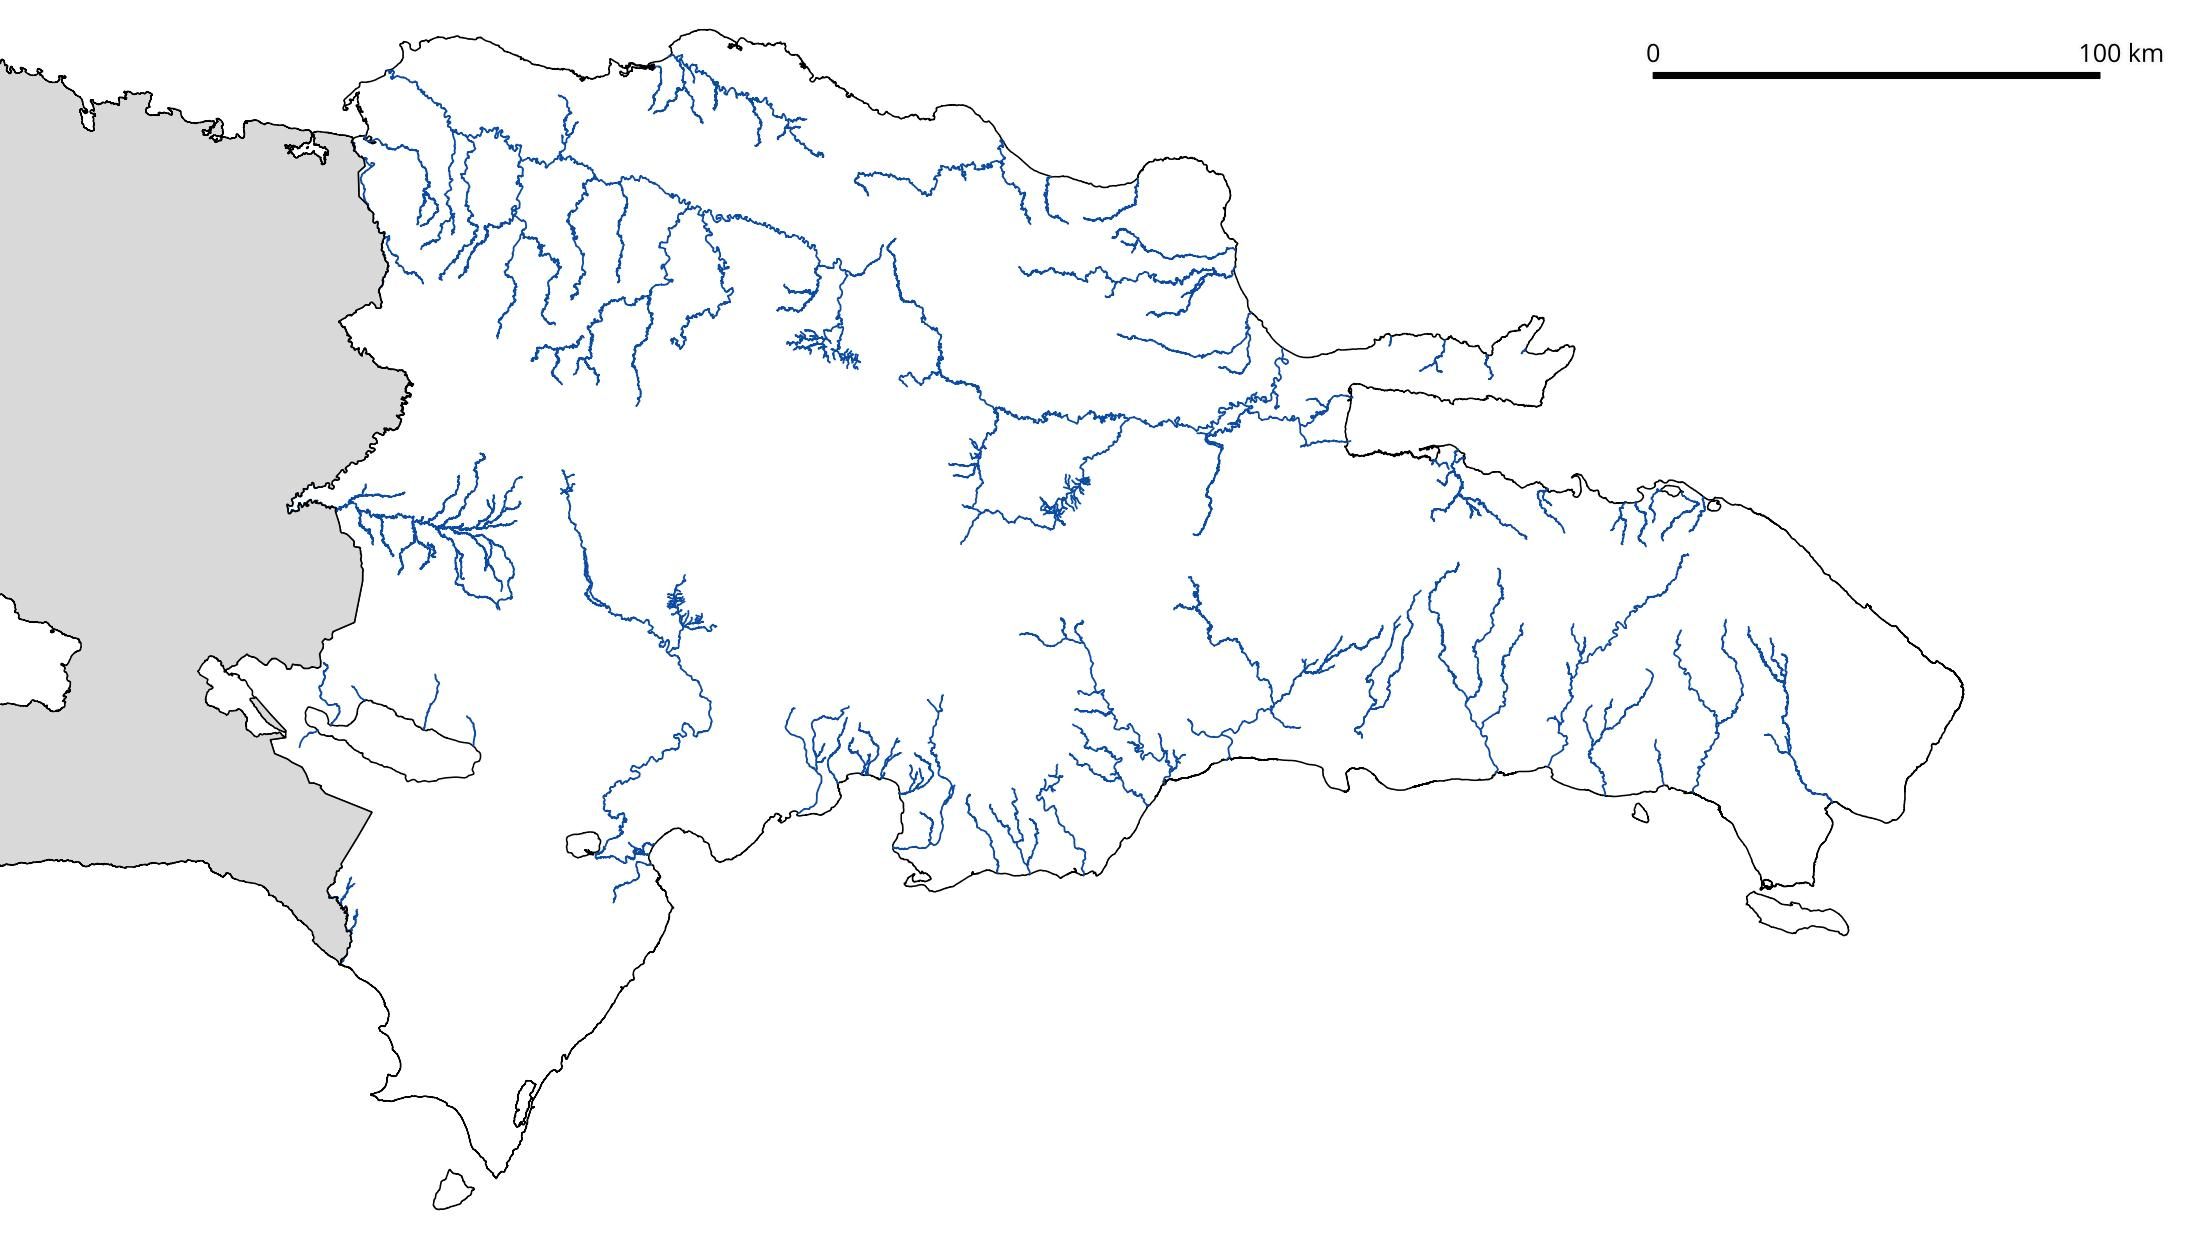
\includegraphics[width=0.8\linewidth]{out/red-cursos-largos} 

}

\caption{Mapa de la red de cursos largos creada para el estudio a partir de varias fuentes (más detalles, en el texto).}\label{fig:redcursoslargos}
\end{figure}

Nuestra de red cursos largos contiene varios ríos que atraviesan amplios
valles y karsts, por lo son comunes los tramos que cruzan zonas
complicadas para la conducción del flujo donde probablemente el error
posicional de las líneas es mayor. Cabe también señalar que, para
asegurar la continuidad topológica de la red, dimos un tratamiento
especial a los ríos que llenan embalses, los cuales representamos por
medio trazados históricos obtenidos del MTN-50K, omitiendo así la
presencia de los embalses.

\begin{Shaded}
\begin{Highlighting}[]
\CommentTok{\# Importar red a GRASS}
\ExtensionTok{v.import} \AttributeTok{{-}{-}overwrite}\NormalTok{ input=red\_mtn50k\_cleaned\_largos.gpkg }\DataTypeTok{\textbackslash{}}
\NormalTok{  output=red\_mtn50k\_cleaned\_largos}
\CommentTok{\# Ver mapa importado en lista (q para salir)}
\ExtensionTok{g.list}\NormalTok{ type=vector}
\CommentTok{\# Calcular y pasar a archivo, la longitud de cursos}
\CommentTok{\# y número de segmentos (ejecutar en casos de actualización)}
\ExtensionTok{v.to.db} \AttributeTok{{-}p}\NormalTok{ option=length map=red\_mtn50k\_cleaned\_largos }\OperatorTok{\textgreater{}} \DataTypeTok{\textbackslash{} }
  \ExtensionTok{stats\_length\_red\_mtn50k\_cleaned\_largos.txt}
\end{Highlighting}
\end{Shaded}

\begin{Shaded}
\begin{Highlighting}[]
\NormalTok{stats\_red\_mtn50k\_largos }\OtherTok{\textless{}{-}} \FunctionTok{read\_delim}\NormalTok{(}
  \FunctionTok{paste0}\NormalTok{(dem\_proc\_dir,}
         \StringTok{\textquotesingle{}stats\_length\_red\_mtn50k\_cleaned\_largos.txt\textquotesingle{}}\NormalTok{),}
  \AttributeTok{progress =}\NormalTok{ F, }\AttributeTok{show\_col\_types =}\NormalTok{ F)}
\NormalTok{n\_seg\_red\_mtn50k\_largos }\OtherTok{\textless{}{-}}\NormalTok{ stats\_red\_mtn50k\_largos }\SpecialCharTok{\%\textgreater{}\%}
  \FunctionTok{filter}\NormalTok{(}\SpecialCharTok{!}\NormalTok{cat}\SpecialCharTok{=={-}}\DecValTok{1}\NormalTok{) }\SpecialCharTok{\%\textgreater{}\%}\NormalTok{ nrow}
\NormalTok{length\_mtn50k\_largos }\OtherTok{\textless{}{-}}\NormalTok{ stats\_red\_mtn50k\_largos }\SpecialCharTok{\%\textgreater{}\%}
  \FunctionTok{filter}\NormalTok{(}\SpecialCharTok{!}\NormalTok{cat}\SpecialCharTok{=={-}}\DecValTok{1}\NormalTok{) }\SpecialCharTok{\%\textgreater{}\%} \FunctionTok{pull}\NormalTok{(length) }\SpecialCharTok{\%\textgreater{}\%}\NormalTok{ sum}\SpecialCharTok{/}\DecValTok{1000}
\end{Highlighting}
\end{Shaded}

Finalmente, importamos nuestra red de cursos largos a la base de datos
de GRASS GIS y generamos estadísticas básicas. Se trata de una red
compuesta por \textbf{1047 segmentos} que suman un total de
\textbf{4895.88 kilómetros} de longitud. Cabe señalar que esta red no
tiene valor hidrográfico, pues, como indicamos, ignora los lagos para
garantizar la integridad topológica. Desaconsejamos su uso para otro fin
que no sea el grabado de un DEM.

El siguiente paso consistió en realizar el \emph{stream burning}
(tallado) de la red de cursos largos con distintos algoritmos sobre el
DEM. Probamos las funciones \texttt{r.carve} y \texttt{r.mapcalc}
(álgebra de mapas) de GRASS GIS, y \texttt{FillBurn} de WhiteboxTools
(GRASS Development Team, 2022a; Lindsay, 2018). Sin embargo, es
importante señalar que, dependiendo del algoritmo usado, el grabado
modifica de forma diferente el DEM. Además, algunos algoritmos modifican
no solamente los píxeles intersectados sino también otros píxeles,
incluso pueden llegar a cambiar los valores en el DEM completo. Nosotros
priorizamos un método de grabado que fuese efectivo pero que a la vez
produjese la mínima alteración sobre el DEM.

Comenzamos con \texttt{r.carve}, una herramienta diseñada para grabar el
DEM sin modificarlo sustancialmente, permitiendo al mismo tiempo
configurar la profundidad y la anchura del grabado (GRASS Development
Team, 2022b; Petrasova et~al., 2011). Por defecto, la anchura de lecho
es equivalente a la resolución del DEM. La profundidad puede definirse
por el usuario, para lo cual nosotros establecimos 100 metros. Pudimos
tallar la red de cursos largos sobre el DEM con esta herramienta,
generando un resultado que consideramos bueno, aunque el proceso ocupó
más de 1 hora de tiempo de cómputo. Esta alternativa es recomendada si
resultase imprescindible conservar las propiedades topográficas en el
DEM, pero debe tenerse en cuenta que su rendimiento es muy bajo. En los
casos en los que se use un DEM de resolución baja, se recomienda usar
esta alternativa. Sin embargo, a nosotros no nos resultó apropiado este
método por razones de rendimiento, que explicamos a continuación. Para
evaluar el rendimiento del DEM tallado, realizábamos un procesamiento
hidrológico abreviado (generación de la acumulación de flujo y
extracción de la red con \texttt{r.watershed}); si los productos
generados (e.g.~red hidrográfica) no nos parecían idóneos, nos veíamos
en la necesidad iterar, editando la red y aplicando el tallado
nuevamente. Dado que el complemento \texttt{r.carve} era poco eficiente,
preferimos buscar otras opciones de tallado.

\begin{Shaded}
\begin{Highlighting}[]
\CommentTok{\# Limpiar red manualmente en QGIS}
\CommentTok{\# Para mejorar la topología, se puede aplicar v.clean directamente en QGIS}

\CommentTok{\# Tallar red de cursos largos}
\BuiltInTok{time}\NormalTok{ r.carve }\AttributeTok{{-}{-}overwrite} \AttributeTok{{-}{-}verbose}\NormalTok{ raster=dem\_pseudo\_ortometrico }\DataTypeTok{\textbackslash{}}
\NormalTok{  vector=red\_mtn50k\_cleaned\_largos output=dem\_tallado depth=100}
\BuiltInTok{echo} \StringTok{"r.carve finalizado"} \KeywordTok{|} \ExtensionTok{mail} \AttributeTok{{-}s} \StringTok{"r.carve finalizado"}\NormalTok{ USUARIO@MAIL}
\CommentTok{\#\# real 97m3.970s}
\end{Highlighting}
\end{Shaded}

Posteriormente, probamos el tallado usando álgebra de mapas con
herramienta \texttt{r.mapcalc} de GRASS GIS (GRASS Development Team,
2022a; GRASS Development Team, 2022c; Larson et~al., 1991; Shapiro y
Westervelt, 1994). Para tallar con álgebra de mapas, primero
normalizamos el DEM, generamos una capa booleana ráster con la red de
cursos largos, la restamos al DEM normalizado y luego, para restablecer
los valores originales fuera de las áreas talladas, multiplicamos el
ráster resultante de la resta nuevamente por el rango del DEM (máximo -
mínimo). El resultado es un DEM tallado, en el que sólo los píxeles por
donde circula la red quedaron con una profundidad equivalente al rango.

\begin{Shaded}
\begin{Highlighting}[]
\CommentTok{\# Limpiar red manualmente en QGIS}
\CommentTok{\# Para mejorar la topología, se puede aplicar v.clean directamente en QGIS}

\CommentTok{\# Tallar}
\CommentTok{\# Rasterizar red (los píxeles de la red valdrán 1, el resto, nulo)}
\NormalTok{v.to.rast }\SpecialCharTok{{-}{-}}\NormalTok{overwrite input}\OtherTok{=}\NormalTok{red\_mtn50k\_cleaned\_largos type}\OtherTok{=}\NormalTok{line use}\OtherTok{=}\NormalTok{val \textbackslash{}}
\NormalTok{  output}\OtherTok{=}\NormalTok{red\_mtn50k\_cleaned\_largos}
\CommentTok{\# Convertir nulos a cero}
\NormalTok{r.null map}\OtherTok{=}\NormalTok{red\_mtn50k\_cleaned\_largos null}\OtherTok{=}\DecValTok{0}
\CommentTok{\# Determinar estadísticas univariantes del DEM}
\NormalTok{r.univar map}\OtherTok{=}\NormalTok{dem\_pseudo\_ortometrico}
\CommentTok{\# minimum: {-}51.4456}
\CommentTok{\# maximum: 3102.34}

\CommentTok{\# Aplicar normalización y resta}
\NormalTok{r.mapcalc }\SpecialCharTok{{-}{-}}\NormalTok{overwrite }\SpecialCharTok{\textless{}}\ErrorTok{\textless{}}\NormalTok{ EOF}
\FunctionTok{eval}\NormalTok{(}\AttributeTok{stddem =}\NormalTok{ (dem\_pseudo\_ortometrico }\SpecialCharTok{{-}} \SpecialCharTok{{-}}\FloatTok{51.4456}\NormalTok{) }\SpecialCharTok{/}\NormalTok{ (}\FloatTok{3102.34} \SpecialCharTok{{-}} \SpecialCharTok{{-}}\FloatTok{51.4456}\NormalTok{), }\SpecialCharTok{\textbackslash{}}
     \AttributeTok{stddemburn =}\NormalTok{ stddem }\SpecialCharTok{{-}}\NormalTok{ red\_mtn50k\_cleaned\_largos)}
\NormalTok{dem\_tallado }\OtherTok{=}\NormalTok{ (stddemburn }\SpecialCharTok{*}\NormalTok{ (}\FloatTok{3102.34} \SpecialCharTok{{-}} \SpecialCharTok{{-}}\FloatTok{51.4456}\NormalTok{)) }\SpecialCharTok{{-}} \FloatTok{51.4456}
\CommentTok{\# dem\_tallado = stddemburn * dem\_pseudo\_ortometrico \# Alternativa}
\NormalTok{EOF}
\NormalTok{echo }\StringTok{"Tallado finalizado"} \SpecialCharTok{|}\NormalTok{ mail }\SpecialCharTok{{-}}\NormalTok{s }\StringTok{"Mensaje sobre tallado"}\NormalTok{ USUARIO}\SpecialCharTok{@}\NormalTok{MAIL}
\end{Highlighting}
\end{Shaded}

\begin{figure}

{\centering \includegraphics[width=0.8\linewidth]{out/dem-sin-tallar-tallado} 

}

\caption{DEM sin aplicación de hidrografía (A), y con aplicación de hidrografía seleccionada (B). El DEM se representa como relieve sombreado y la aplicación se denota como un grabado oscurecido (cañón del río Payabo, Los Haitises, y río Yuna (proximidades de Arenoso, nordeste de República Dominicana)}\label{fig:demtallado}
\end{figure}

Como última alternativa de procesamiento, probamos la herramienta
\texttt{FillBurn}, basada en Saunders (2000) e implementada por Lindsay
(2016) en de WBT. \texttt{FillBurn} realiza dos modificaciones a la vez
sobre el DEM; por una parte, graba la red, usando una profundidad por
defecto y, por otro, rellena las depresiones. La herramienta mostró
mejor rendimiento que la de GRASS GIS en cuanto a tiempo de cómputo.
Tras tallar la red evaluamos el DEM resultante, y comprobamos que
\textbf{resultó ser muy diferente al original, especialmente en las
áreas con depresiones}. Por esta razón, descartamos este DEM y elegimos
usar el tallado por medio de álgebra de mapas (\texttt{r.mapcalc}) con
GRASS GIS en los siguientes pasos de nuestro flujo de trabajo.

\begin{Shaded}
\begin{Highlighting}[]
\CommentTok{\# Exportar dem\_pseudo\_ortometrico a GTiff con compresión LZW}
\BuiltInTok{time}\NormalTok{ r.out.gdal }\AttributeTok{{-}{-}overwrite} \AttributeTok{{-}{-}verbose}\NormalTok{ createopt=}\StringTok{"COMPRESS=LZW,BIGTIFF=YES"} \DataTypeTok{\textbackslash{}}
\NormalTok{ input=dem\_pseudo\_ortometrico }\DataTypeTok{\textbackslash{}}
\NormalTok{ format=GTiff type=Float64 output=dem\_pseudo\_ortometrico.tif}
\BuiltInTok{echo} \StringTok{"Job finished"} \KeywordTok{|} \ExtensionTok{mail} \AttributeTok{{-}s} \StringTok{"Job finished"}\NormalTok{ USUARIO@MAIL}
\CommentTok{\#\# real 1m0.248s}

\CommentTok{\# Exportar red\_mtn50k\_cleaned\_largos.gpkg a shapefile}
\ExtensionTok{ogr2ogr}\ErrorTok{(}
  \ExtensionTok{src\_datasource\_name}\NormalTok{ = }\StringTok{\textquotesingle{}/media/jose/datos/alos{-}palsar{-}dem{-}rd/dem/red\_mtn50k\_cleaned\_largos.gpkg\textquotesingle{}}\NormalTok{,}
  \ExtensionTok{dst\_datasource\_name}\NormalTok{ = }\StringTok{\textquotesingle{}/media/jose/datos/alos{-}palsar{-}dem{-}rd/dem/red\_mtn50k\_cleaned\_largos.shp\textquotesingle{}}\NormalTok{,}
  \VariableTok{verbose}\OperatorTok{=}\NormalTok{TRUE}\KeywordTok{)}

\CommentTok{\# Tallar con WBT}
\BuiltInTok{time}\NormalTok{ \textasciitilde{}/WhiteboxTools\_linux\_amd64/WBT/whitebox\_tools }\DataTypeTok{\textbackslash{}}
  \AttributeTok{{-}{-}wd}\OperatorTok{=}\StringTok{\textquotesingle{}/media/jose/datos/alos{-}palsar{-}dem{-}rd/dem/\textquotesingle{}} \DataTypeTok{\textbackslash{}}
  \AttributeTok{{-}{-}run}\OperatorTok{=}\NormalTok{FillBurn }\AttributeTok{{-}{-}dem}\OperatorTok{=}\StringTok{\textquotesingle{}dem\_pseudo\_ortometrico.tif\textquotesingle{}} \DataTypeTok{\textbackslash{}}
  \AttributeTok{{-}{-}streams}\OperatorTok{=}\NormalTok{red\_mtn50k\_cleaned.shp }\AttributeTok{{-}{-}output}\OperatorTok{=}\StringTok{\textquotesingle{}dem\_tallado.tif\textquotesingle{}} \AttributeTok{{-}v}
\BuiltInTok{echo} \StringTok{"Job finished"} \KeywordTok{|} \ExtensionTok{mail} \AttributeTok{{-}s} \StringTok{"Job finished"}\NormalTok{ USUARIO@MAIL}
\CommentTok{\#\# real 9m21.980s}
\CommentTok{\# Importar a GRASS GIS}
\BuiltInTok{time}\NormalTok{ r.import }\AttributeTok{{-}{-}overwrite}\NormalTok{ input=dem\_tallado.tif output=dem\_tallado}
\BuiltInTok{echo} \StringTok{"Job finished"} \KeywordTok{|} \ExtensionTok{mail} \AttributeTok{{-}s} \StringTok{"Job finished"}\NormalTok{ USUARIO@MAIL}
\CommentTok{\#\# real 0m38.519s}
\end{Highlighting}
\end{Shaded}

A continuación, aplicamos algoritmos de grabado de depresiones \ldots{}
\ldots{} \ldots{}

\hypertarget{procesamiento-de-hidrologuxeda-computacional-1}{%
\subsubsection{Procesamiento de hidrología
computacional}\label{procesamiento-de-hidrologuxeda-computacional-1}}

El próximo paso consistió en

\hypertarget{informe-de-la-sesiuxf3n-de-r}{%
\subsection*{Informe de la sesión de
R}\label{informe-de-la-sesiuxf3n-de-r}}
\addcontentsline{toc}{subsection}{Informe de la sesión de R}

\begin{Shaded}
\begin{Highlighting}[]
\FunctionTok{sessionInfo}\NormalTok{()}
\end{Highlighting}
\end{Shaded}

\begin{verbatim}
## R version 4.3.0 (2023-04-21)
## Platform: x86_64-pc-linux-gnu (64-bit)
## Running under: Ubuntu 20.04.3 LTS
## 
## Matrix products: default
## BLAS:   /usr/lib/x86_64-linux-gnu/blas/libblas.so.3.9.0 
## LAPACK: /usr/lib/x86_64-linux-gnu/lapack/liblapack.so.3.9.0
## 
## locale:
##  [1] LC_CTYPE=es_DO.UTF-8       LC_NUMERIC=C              
##  [3] LC_TIME=es_DO.UTF-8        LC_COLLATE=es_DO.UTF-8    
##  [5] LC_MONETARY=es_DO.UTF-8    LC_MESSAGES=es_DO.UTF-8   
##  [7] LC_PAPER=es_DO.UTF-8       LC_NAME=C                 
##  [9] LC_ADDRESS=C               LC_TELEPHONE=C            
## [11] LC_MEASUREMENT=es_DO.UTF-8 LC_IDENTIFICATION=C       
## 
## time zone: America/Santo_Domingo
## tzcode source: system (glibc)
## 
## attached base packages:
## [1] stats     graphics  grDevices utils     datasets  methods   base     
## 
## other attached packages:
##  [1] gdalUtilities_1.2.4 lubridate_1.9.2     forcats_1.0.0      
##  [4] stringr_1.5.0       dplyr_1.1.2         purrr_1.0.1        
##  [7] readr_2.1.4         tidyr_1.3.0         tibble_3.2.1       
## [10] ggplot2_3.4.2       tidyverse_2.0.0     kableExtra_1.3.4   
## [13] sf_1.0-12           raster_3.6-20       sp_1.6-0           
## 
## loaded via a namespace (and not attached):
##  [1] gtable_0.3.3       xfun_0.39          lattice_0.20-45    tzdb_0.4.0        
##  [5] vctrs_0.6.2        tools_4.3.0        generics_0.1.3     parallel_4.3.0    
##  [9] proxy_0.4-27       fansi_1.0.4        pkgconfig_2.0.3    Matrix_1.4-0      
## [13] KernSmooth_2.23-20 webshot_0.5.4      lifecycle_1.0.3    compiler_4.3.0    
## [17] munsell_0.5.0      terra_1.7-29       codetools_0.2-18   htmltools_0.5.5   
## [21] class_7.3-20       yaml_2.3.7         crayon_1.5.2       pillar_1.9.0      
## [25] classInt_0.4-9     tidyselect_1.2.0   rvest_1.0.3        digest_0.6.31     
## [29] stringi_1.7.12     fastmap_1.1.1      grid_4.3.0         colorspace_2.1-0  
## [33] cli_3.6.1          magrittr_2.0.3     utf8_1.2.3         e1071_1.7-13      
## [37] withr_2.5.0        scales_1.2.1       bit64_4.0.5        timechange_0.2.0  
## [41] rmarkdown_2.21     httr_1.4.6         bit_4.0.5          reticulate_1.30   
## [45] hms_1.1.3          png_0.1-8          evaluate_0.21      knitr_1.42        
## [49] viridisLite_0.4.2  rticles_0.25       rlang_1.1.1        Rcpp_1.0.10       
## [53] glue_1.6.2         DBI_1.1.3          xml2_1.3.4         vroom_1.6.3       
## [57] svglite_2.1.1      rstudioapi_0.14    jsonlite_1.8.4     R6_2.5.1          
## [61] systemfonts_1.0.4  units_0.8-2
\end{verbatim}

\hypertarget{referencias}{%
\section*{Referencias}\label{referencias}}
\addcontentsline{toc}{section}{Referencias}

\hypertarget{refs}{}
\begin{CSLReferences}{1}{0}
\leavevmode\vadjust pre{\hypertarget{ref-anderson2010geomorphology}{}}%
Anderson, R. S. y Anderson, S. P. (2010). \emph{Geomorphology: the
mechanics and chemistry of landscapes}. Cambridge University Press.

\leavevmode\vadjust pre{\hypertarget{ref-asfdaac2014hires}{}}%
ASF DAAC. (2014).
\emph{PALSAR{\_}Radiometric{\_}Terrain{\_}Corrected{\_}high{\_}res}.
\url{https://doi.org/10.5067/Z97HFCNKR6VA}

\leavevmode\vadjust pre{\hypertarget{ref-aziz2022}{}}%
Aziz, K. M. A. y Rashwan, K. S. (2022). Comparison of different
resolutions of six free online DEMs with GPS elevation data on a new 6th
of October City, Egypt. \emph{Arabian Journal of Geosciences},
\emph{15}(20), 1585. \url{https://doi.org/10.1007/s12517-022-10845-5}

\leavevmode\vadjust pre{\hypertarget{ref-burn1997}{}}%
Burn, D. H. (1997). Hydrological information for sustainable
development. \emph{Hydrological Sciences Journal}, \emph{42}(4),
481-492. \url{https://doi.org/10.1080/02626669709492048}

\leavevmode\vadjust pre{\hypertarget{ref-charlton2010fundamentals}{}}%
Charlton, R. (2010). \emph{Fundamentals of fluvial geomorphology}
(Repr). Routledge.

\leavevmode\vadjust pre{\hypertarget{ref-cidiatindrhi1992control}{}}%
CIDIAT y INDRHI. (1992). \emph{{Control de Inundaciones en la cuenca del
Río Yaque del Sur}}. {Instituto Nacional de Recursos Hidráulicos
(INDRHI)}.

\leavevmode\vadjust pre{\hypertarget{ref-foucault1985diccionario}{}}%
Foucault, A. y Raoult, J. F. (1985). \emph{Diccionario de Geología}.
MASSON. \url{https://books.google.com.do/books?id=x5FDPQAACAAJ}

\leavevmode\vadjust pre{\hypertarget{ref-gadm}{}}%
GADM. (2022). \emph{{GADM}}. Available online:
\url{https://gadm.org/index.html} (accessed on abril, 2023).

\leavevmode\vadjust pre{\hypertarget{ref-garcia2011clasificacion}{}}%
García, J. H. G. y Ojeda, A. O. (2011). Clasificación geomorfológica de
cursos fluviales a partir de sistemas de información geográfica (SIG).
\emph{Boletín de la Asociación de Geógrafos Españoles}, \emph{56},
373-396.

\leavevmode\vadjust pre{\hypertarget{ref-gdal2022gdal}{}}%
GDAL/OGR contributors. (2022). \emph{{GDAL/OGR} Geospatial Data
Abstraction software Library}. Open Source Geospatial Foundation.
\url{https://doi.org/10.5281/zenodo.5884351}

\leavevmode\vadjust pre{\hypertarget{ref-googlemaps}{}}%
Google; Airbus, CNES; Airbus, Landsat; Copernicus; Maxar Technologies;
U.S. Geological Survey. (2023). \emph{Google Maps}.
\url{https://www.google.com/maps/}

\leavevmode\vadjust pre{\hypertarget{ref-GRASS_GIS_software}{}}%
GRASS Development Team. (2022a). \emph{Geographic Resources Analysis
Support System (GRASS) Software, Version 8.0.2}. Open Source Geospatial
Foundation. \url{https://grass.osgeo.org}

\leavevmode\vadjust pre{\hypertarget{ref-grassdev2022rcarve}{}}%
GRASS Development Team. (2022b). \emph{r.carve. Generates stream
channels. Takes vector stream data, transforms it to raster and
subtracts depth from the output DEM. GRASS GIS manual}.
\url{https://grass.osgeo.org/grass82/manuals/r.carve.html}

\leavevmode\vadjust pre{\hypertarget{ref-grassdev2022rmapcalc}{}}%
GRASS Development Team. (2022c). \emph{r.mapcalc - Raster map
calculator. GRASS GIS manual}.
\url{https://grass.osgeo.org/grass82/manuals/r.mapcalc.html}

\leavevmode\vadjust pre{\hypertarget{ref-GRASS_GIS_softwarev82}{}}%
GRASS Development Team. (2023). \emph{Geographic Resources Analysis
Support System (GRASS) Software, Version 8.2.0}. Open Source Geospatial
Foundation. \url{https://grass.osgeo.org}

\leavevmode\vadjust pre{\hypertarget{ref-gutierrez2009geomorfologia}{}}%
Gutiérrez Elorza, M. (2009). \emph{Geomorfología} (Última reimpr).
Pearson-Prentice Hall.

\leavevmode\vadjust pre{\hypertarget{ref-halcrow1992estudio}{}}%
Halcrow-COR Ing. S.A. (2002). \emph{{Estudio de Vulnerabilidad de las
Grandes Presas}}. {Instituto Nacional de Recursos Hidráulicos (INDRHI)}.

\leavevmode\vadjust pre{\hypertarget{ref-hijmans2023raster}{}}%
Hijmans, R. J. (2023). \emph{raster: Geographic Data Analysis and
Modeling}. \url{https://CRAN.R-project.org/package=raster}

\leavevmode\vadjust pre{\hypertarget{ref-indrhi1996estadisticas}{}}%
INDRHI. (1996). \emph{{Estadísticas del Agua en la República
Dominicana}}. {Instituto Nacional de Recursos Hidráulicos (INDRHI)}.

\leavevmode\vadjust pre{\hypertarget{ref-indrhi2012plan}{}}%
INDRHI. (2012). \emph{{Plan Hidrológico Nacional, República
Dominicana}}. {Instituto Nacional de Recursos Hidráulicos (INDRHI)}.

\leavevmode\vadjust pre{\hypertarget{ref-indrhi2019inventario}{}}%
INDRHI. (2019). \emph{{Inventario de Estaciones Hidrometeorológicas.
Informe Final}}. {Instituto Nacional de Recursos Hidráulicos}.

\leavevmode\vadjust pre{\hypertarget{ref-indrhiaquater2000estudio}{}}%
INDRHI y AQUATER. (2000). \emph{{Estudio Hidrogeológico Nacional de la
República Dominicana, Fase I. Memoria de Proyecto, 7 volúmenes}}.
{Instituto Nacional de Recursos Hidráulicos (INDRHI)}.

\leavevmode\vadjust pre{\hypertarget{ref-indrhieptisa2004estudio}{}}%
INDRHI y EPTISA. (2000). \emph{{Estudio Hidrogeológico Nacional de la
República Dominicana, Fase II}}. {Instituto Nacional de Recursos
Hidráulicos (INDRHI)}.

\leavevmode\vadjust pre{\hypertarget{ref-icm1989serie}{}}%
Instituto Cartográfico Militar (ICM). (1989). \emph{{Serie E733 de mapas
topográficos escala 1:50,000}}. {Instituto Cartográfico Militar}.

\leavevmode\vadjust pre{\hypertarget{ref-ign2022medicion}{}}%
Instituto Geográfico Nacional. (2022). \emph{Medición por Sistema Global
de Navegación por Satélite (GNSS) de los Tres Picos Más Altos De Las
Antillas}. Disponible en línea. Accedido a través de
\url{https://www.ign.gob.do/index.php/noticias/item/448-medicion-por-sistema-global-de-navegacion-por-satelite-gnss-de-los-tres-picos-mas-altos-de-las-antillas}.

\leavevmode\vadjust pre{\hypertarget{ref-Izzo2010ANC}{}}%
Izzo, M., Rosskopf, C. M., Aucelli, P. P. C., Maratea, A., Méndez, R.
E., Pérez, C. y Segura, H. (2010). A New Climatic Map of the Dominican
Republic Based on the Thornthwaite Classification. \emph{Physical
Geography}, \emph{31}, 455-472.

\leavevmode\vadjust pre{\hypertarget{ref-jarvis2008}{}}%
Jarvis, A., Reuter, H. I., Nelson, A. y Guevara, E. (2008). Hole-filled
SRTM for the globe Version 4. \emph{available from the CGIAR-CSI SRTM
90m Database (http://srtm. csi. cgiar. org)}, \emph{15}(25-54), 5.

\leavevmode\vadjust pre{\hypertarget{ref-jaxameti2007alos}{}}%
JAXA/METI y ASF DAAC. (2015). \emph{{ALOS
PALSAR\_Radiometric\_Terrain\_Corrected\_high\_res. Includes material de
JAXA/METI 2010}}. Disponible en línea. Accedido a través de ASF DAAC
\url{https://asf.alaska.edu/}. DOI:
\url{https://doi.org/10.5067/Z97HFCNKR6VA} (accessed on abril, 2023).

\leavevmode\vadjust pre{\hypertarget{ref-larson1991performing}{}}%
Larson, M., Shapiro, M. y Tweddale, S. (1991). Performing map
calculations on GRASS data: r. mapcalc program tutorial. \emph{US Army
Corps of Engineers, Construction Engineering Research Laboratory.
https://grass. osgeo. org/uploads/grass/history{\_}docs/mapcalc. pdf}.

\leavevmode\vadjust pre{\hypertarget{ref-Le2019ClimateCA}{}}%
Le, T. D. N. (2019). Climate change adaptation in coastal cities of
developing countries: characterizing types of vulnerability and
adaptation options. \emph{Mitigation and Adaptation Strategies for
Global Change}, \emph{25}, 739-761.

\leavevmode\vadjust pre{\hypertarget{ref-LincolnLenderking2020ClimateCA}{}}%
Lenderking, H. L., Robinson, S. y Carlson, G. R. (2020). Climate change
and food security in Caribbean small island developing states:
challenges and strategies. \emph{International Journal of Sustainable
Development \& World Ecology}, \emph{28}, 238-245.

\leavevmode\vadjust pre{\hypertarget{ref-lindsay2016}{}}%
Lindsay, J. B. (2016). The practice of DEM stream burning revisited: The
Practice of DEM Stream Burning Revisited. \emph{Earth Surface Processes
and Landforms}, \emph{41}(5), 658-668.
\url{https://doi.org/10.1002/esp.3888}

\leavevmode\vadjust pre{\hypertarget{ref-lindsay2018whiteboxtools}{}}%
Lindsay, J. B. (2018). \emph{{WhiteboxTools user manual}}. Available
online: \url{https://www.whiteboxgeo.com/manual/wbt_book/intro.html}
(accessed on abril, 2023).

\leavevmode\vadjust pre{\hypertarget{ref-lindsay2019}{}}%
Lindsay, J. B., Francioni, A. y Cockburn, J. M. H. (2019). LiDAR DEM
Smoothing and the Preservation of Drainage Features. \emph{Remote
Sensing}, \emph{11}(16), 1926. \url{https://doi.org/10.3390/rs11161926}

\leavevmode\vadjust pre{\hypertarget{ref-Lohmann2016ComparingVA}{}}%
Lohmann, H. (2016). Comparing vulnerability and adaptive capacity to
climate change in individuals of coastal Dominican Republic. \emph{Ocean
\& Coastal Management}, \emph{132}, 111-119.

\leavevmode\vadjust pre{\hypertarget{ref-Mackay2017TheFO}{}}%
Mackay, E. A. y Spencer, A. J. (2017). The future of Caribbean tourism:
competition and climate change implications. \emph{Worldwide Hospitality
and Tourism Themes}, \emph{9}, 44-59.

\leavevmode\vadjust pre{\hypertarget{ref-martinez2023datos}{}}%
Martínez-Batlle, J.-R. y Izzo-Gioiosa, M. (2023). \emph{Datos del
estudio "Generación de red hidrográfica densa de República Dominicana a
partir de modelo digital de elevaciones de resolución media"}.
\url{https://doi.org/10.5281/ZENODO.8146391}

\leavevmode\vadjust pre{\hypertarget{ref-mishra2009}{}}%
Mishra, A. K. y Coulibaly, P. (2009). Developments in hydrometric
network design: A review. \emph{Reviews of Geophysics}, \emph{47}(2),
RG2001. \url{https://doi.org/10.1029/2007RG000243}

\leavevmode\vadjust pre{\hypertarget{ref-mishra2010}{}}%
Mishra, A. K. y Coulibaly, P. (2010). Hydrometric network evaluation for
Canadian watersheds. \emph{Journal of Hydrology}, \emph{380}(3-4),
420-437. \url{https://doi.org/10.1016/j.jhydrol.2009.11.015}

\leavevmode\vadjust pre{\hypertarget{ref-nasajpl2013nasa}{}}%
NASA JPL. (2013). \emph{NASA Shuttle Radar Topography Mission Global 3
arc second {[}Data set{]}}.
\url{https://doi.org/10.5067/MEaSUREs/SRTM/SRTMGL3.003}

\leavevmode\vadjust pre{\hypertarget{ref-nasa2014srtm1sdem}{}}%
NASA LP DAAC. (2000). \emph{SRTM 1 Arc-Second Global}.
\url{https://earthexplorer.usgs.gov/}.

\leavevmode\vadjust pre{\hypertarget{ref-nasa2013aster}{}}%
National Aeronautics and Space Administration y United States Geological
Survey. (2009). \emph{{ASTER GDEM}}. \url{https://lpdaac.usgs.gov/}.

\leavevmode\vadjust pre{\hypertarget{ref-obrien2023gdalutilities}{}}%
O'Brien, J. (2023). \emph{gdalUtilities: Wrappers for 'GDAL' Utilities
Executables}. \url{https://CRAN.R-project.org/package=gdalUtilities}

\leavevmode\vadjust pre{\hypertarget{ref-ocha2023hdx}{}}%
OCHA. (2022). \emph{{Humanitarian Data Exchange (OCHA)}}. Available
online: \url{https://data.humdata.org/dataset/cod-ab-dom} (accessed on
abril, 2023).

\leavevmode\vadjust pre{\hypertarget{ref-oeaindrhi1994estudio}{}}%
OEA y INDRHI. (1994). \emph{{Plan Nacional de Ordenamiento de los
Recursos Hídricos (PNORHI)}}. {Instituto Nacional de Recursos
Hidráulicos (INDRHI)}.

\leavevmode\vadjust pre{\hypertarget{ref-one2023division}{}}%
Oficina Nacional de Estadística (ONE). (2018). \emph{{División
territorial de República Dominicana}}. Available online:
\url{https://www.one.gob.do/media/s5gdl00n/divisi\%C3\%B3n-territorial-2020-t.pdf}
(accessed on abril, 2023).

\leavevmode\vadjust pre{\hypertarget{ref-OpenStreetMap}{}}%
OpenStreetMap contributors. (2017). \emph{{Planet dump retrieved from
https://planet.osm.org }}. Available online:
\url{https://www.openstreetmap.org} (accessed on abril, 2023).

\leavevmode\vadjust pre{\hypertarget{ref-pebesma2018simple}{}}%
Pebesma, E. (2018). {Simple Features for R: Standardized Support for
Spatial Vector Data}. \emph{{The R Journal}}, \emph{10}(1), 439-446.
\url{https://doi.org/10.32614/RJ-2018-009}

\leavevmode\vadjust pre{\hypertarget{ref-pebesma2023spatial}{}}%
Pebesma, E. y Bivand, R. (2023). \emph{{Spatial Data Science: With
applications in R}} (p. 352). {Chapman and Hall/CRC}.
\url{https://r-spatial.org/book/}

\leavevmode\vadjust pre{\hypertarget{ref-pedraza1996geomorfologia}{}}%
Pedraza Gilsanz, J. de. (1996). \emph{Geomorfología: principios, métodos
y aplicaciones}. Ed. Rueda.

\leavevmode\vadjust pre{\hypertarget{ref-petrasova2011geoinformation}{}}%
Petrasova, A., Petras, V., Jeziorska, J., White, C. H. C., Reckling, W.,
Millar, G., Grokhowsky, N., Paulukonis, A., Montgomery, K., Coffer, M.,
Harmon, B., Cepero, K., Starek, M., Hardin, N. L. E., Paris, P., Russ,
E., Weaver, K., Fogleman, B., Leo, M. di y Stopkova, E. (2011).
\emph{GeoInformation Science and Environmental Modeling}.
\url{http://fatra.cnr.ncsu.edu/~hmitaso/}

\leavevmode\vadjust pre{\hypertarget{ref-QGIS_software}{}}%
QGIS Development Team. (2021). \emph{QGIS Geographic Information System,
Version 3.26.2}. QGIS Association. \url{https://www.qgis.org}

\leavevmode\vadjust pre{\hypertarget{ref-rcoreteam2023r}{}}%
R Core Team. (2023). \emph{R: A Language and Environment for Statistical
Computing}. R Foundation for Statistical Computing.
\url{https://www.R-project.org/}

\leavevmode\vadjust pre{\hypertarget{ref-rodriguez2006potencial}{}}%
Rodríguez, H. y Febrillet, J. F. (2006). {Potencial idrogeológico de la
República Dominicana}. \emph{Boletín Geológico y Minero}, \emph{117}.

\leavevmode\vadjust pre{\hypertarget{ref-Roson2013AMF}{}}%
Roson, R. (2013). A Modeling Framework to Assess the Economic Impact of
Climate Change in the Caribbean. \emph{Cepal Review}, \emph{111}, 23-36.

\leavevmode\vadjust pre{\hypertarget{ref-saunders2000}{}}%
Saunders, W. (2000). Preparation of DEMs for use in environmental
modeling analysis. \emph{Hydrologic and Hydraulic Modeling Support.
Redlands, CA: ESRI}, 2951.

\leavevmode\vadjust pre{\hypertarget{ref-semarn2004atlas}{}}%
Secretaría de Estado de Medio Ambiente y Recursos Naturales. (2004).
\emph{{Atlas de los Recursos Naturales de la República Dominicana}}.
{Secretaría de Estado de Medio Ambiente y Recursos Naturales}.

\leavevmode\vadjust pre{\hypertarget{ref-sercitecindrhi2002control}{}}%
SERCITEC y INDRHI. (2002). \emph{{Control de Inundaciones de la cuenca
del Río Yaque del Norte}}. {Instituto Nacional de Recursos Hidráulicos
(INDRHI)}.

\leavevmode\vadjust pre{\hypertarget{ref-shapiro1994rmapcalc}{}}%
Shapiro, M. y Westervelt, J. (1994). \emph{r. mapcalc: An algebra for
GIS and image processing}. US Army Corps of Engineers, Construction
Engineering Research Laboratories.

\leavevmode\vadjust pre{\hypertarget{ref-vanrossum2009python}{}}%
Van Rossum, G. y Drake, F. L. (2009). \emph{Python 3 Reference Manual}.
CreateSpace.

\leavevmode\vadjust pre{\hypertarget{ref-whicham2019welcome}{}}%
Wickham, H., Averick, M., Bryan, J., Chang, W., McGowan, L. D.,
François, R., Grolemund, G., Hayes, A., Henry, L., Hester, J., Kuhn, M.,
Pedersen, T. L., Miller, E., Bache, S. M., Müller, K., Ooms, J.,
Robinson, D., Seidel, D. P., Spinu, V., \ldots{} Yutani, H. (2019).
Welcome to the {tidyverse}. \emph{Journal of Open Source Software},
\emph{4}(43), 1686. \url{https://doi.org/10.21105/joss.01686}

\leavevmode\vadjust pre{\hypertarget{ref-xie2014implementing}{}}%
Xie, Y. (2014). knitr: A Comprehensive Tool for Reproducible Research in
{R}. En V. Stodden, F. Leisch, y R. D. Peng (Eds.), \emph{Implementing
Reproducible Computational Research}. Chapman; Hall/CRC.

\leavevmode\vadjust pre{\hypertarget{ref-xie2015dynamic}{}}%
Xie, Y. (2015). \emph{Dynamic Documents with {R} and knitr} (2nd ed.).
Chapman; Hall/CRC. \url{https://yihui.org/knitr/}

\leavevmode\vadjust pre{\hypertarget{ref-xie2023knitr}{}}%
Xie, Y. (2023). \emph{knitr: A General-Purpose Package for Dynamic
Report Generation in R}. \url{https://yihui.org/knitr/}

\leavevmode\vadjust pre{\hypertarget{ref-zhu2021kableextra}{}}%
Zhu, H. (2021). \emph{kableExtra: Construct Complex Table with 'kable'
and Pipe Syntax}. \url{https://CRAN.R-project.org/package=kableExtra}

\end{CSLReferences}

\bibliographystyle{unsrt}
\bibliography{references.bib}


\end{document}
